\chapter[Open problem and perspectives]{Open problems and perspectives}\label{chp5_opening}
\chaptermark{Open problems and perspectives}

\objectif{
 This final chapter is dedicated to the study of large-population
limits of some general discrete-time epidemics processes.
 We introduce a ``layered''
configuration model as a mathematical framework for understanding the spread of infectious diseases. Building on the inherent versatility of configuration models, our model incorporates a multitype structure by endowing edges with an integer length encoding transmission delays. Through coupling with multitype branching processes on countable state spaces relying on the theoretical limit theorems for Galton--Watson processes with countable types derived in Chapter~\ref{chp2_ks_countable}, we analyze the dynamics and emergence of geodesics. Our main results establish conditions under which the successive times of infection between distinguished focal vertices converge weakly to the atoms of a Cox point process with a characterized intensity.
}

\section{Emergence of $\Lambda$-coalescents from structured interacting population models}
In this first part of the opening chapter, we offer a heuristic of how the methodology developed in Section~\ref{sec:many_to_few} of Chapter~\ref{chp4_multitype} could easily be generalized to a wider class of regulated models with a finite set of types. In particular, we think that the methodology carried out in this article can be easily used to extend the universality class of $\Lambda$-coalescents to regulated particle models on finite type spaces. 
 Looking back at the proof of Theorem~\ref{thm:main_multitype}, we used extensively the second moment assumption in Assumption~\ref{hyp:kingman}: first in Section~\ref{sec:ch4_calcul_sto} to obtain convergence of the type-frequeny process and the re-scaled subfamilies on the timescale $O(K)$ to the stable equilibrium $\tilde h$, and then in Section~\ref{sec:convergence_semigroup} to obtain the convergence of the Feynman--Kac term to the probability of maintaining $k$ distinct lineages in the $k$-Kingman coalescent. In particular, the second moment assumption was crucial in the proof of Lemma~\ref{lem:GH/H} to derive the limit of $K\mathcal{G}^k\bm{1}( \mathcal{Z}^k_{Kt},\bm S^k_{Kt})$ as $K\to\infty$. In particular we only needed to do a asymptotic expansion of $\mathcal{H}$ up to the second order, and the second moment assumption ensured that the remainder term was negligible.


 Now, assume that we relax the second moment assumption in Assumption~\ref{hyp:kingman} to a weaker heavy tail condition on the offspring distribution. As in~\citet{schweinsberg2003coalescent}, let us assume that exists some parameter $\alpha\in (1,2)$ such that for all $x\in E$, $z\in \mathscr{B}_{\eps}$,
  \begin{equation}\label{eq:heavy_tail_condition}
 \Prob\big(L(z)\geq k\big)\ \sim\ Ck^{-\alpha}.
 \end{equation} 
From there, we obtain that for $d\in\{2,\ldots,k\}$, the truncated moment of order $d\geq 2$ asymptotically scales like $K^{d-\alpha}$:
  \begin{equation}\label{eq:estimation_moment_heavytail}
 M^d_K(z)\ \coloneqq\ \E\big[\lVert L(z)\rVert^d\1(\lVert L(z)\rVert\leq K)\big]\ \sim\ K^{d-\alpha}.
 \end{equation} 

 For $p\in \N$, denote by $D^p$ the derivation operator to the order $p$.
For every $y\in E$ and $n\in \N^E$, the asymptotic expansion of the function
\[
t\ \longmapsto\ \mathcal{H}\Big(z+t\frac{n-e_y}{K},\bm x\Big)
\]
made in Chapter~\ref{chp4_multitype} pushed to order $k$ writes as

\[
\mathcal{H}\Big( z+\frac{n-e_y}{K},\bm x\Big) \ =\ \sum_{d=0}^k \frac{1}{d!}D^d\mathcal{H}( z,\bm x)\Big[\frac{n-e_y}{K}\Big]^d
 + R_{k+1}\Big(z,\frac{n-e_y}{K}\Big).
\]
Using as in Chapter~\ref{chp4_multitype} the integral remainder Taylor formula, remainder term writes as
\begin{equation}\label{eq:reste_order_k}
R_{k+1}\Big(z,\frac{n-e_y}{K}\Big)\ \coloneqq\ \int_0^1\frac{1-t}{k! K^k}\Big[D^{k}\mathcal{H}(z+s \frac{n-e_y}{K}, \bm x)- D^{k}\mathcal{H}(z,\bm x)\Big]\Big[\frac{n-e_y}{K}\Big]^{k}.
\end{equation}

We still have that under $\Prob^0$, $\Delta \bm z^{i_1}_{x_1}\cdots\Delta \bm z^{i_d}_{x_d}=0$  if there exists $d_1, d_2$ such that $i_{c_1}\neq i_{d_2}$ and $\partial^2_{(i,x),(i,y)}\mathcal{H}^k(\bm z)=0$ for $i>0$. It follows that the only non-zero terms in the expansion are those for which  $i_1= \cdots = i_d=0$ or all but one are zero. Therefore, for $z\in\mathscr{B}_{\eps}$ and $\bm x\in E^k$, the asymptotic development of $\mathcal{G}^k\bm{1}(z,\bm x)$  would be of the form 
\begin{multline*}
\mathcal{G}^k\bm{1}(z, \bm x)\ =\  \sum_{d=0}^k \sum_{x_1, \ldots, x_d} \frac{\partial^d_{(0, x_1),\ldots, (0, x_d)}\mathcal{H}^k(\bm z)}{\mathcal{H}^k(\bm z)}\E^0\Big[\prod_{p=1}^d \Delta z_{x_p}\Big]  \\ + d \sum_{i=1}^k \sum_{x_1, \ldots, x_d}\frac{\partial^d_{(i, x_1),\ldots, (0, x_d)}\mathcal{H}^k(\bm z)}{\mathcal{H}^k(\bm z)} \E^0\Big[\prod_{p=1}^d \Delta z^i_{x_p}\Big]. 
\end{multline*}

By the generalized Leibniz formula,
we have that for $d\in\{1,\ldots, k\}$ and $x_1, \ldots, x_d\in E$,
\[
\frac{1}{\mathcal{H}^k(\bm z)}\partial^d_{(0, x_1),\ldots, (0, x_d)}\mathcal{H}^k(\bm z)\ =\ \sum_{(A_1, \ldots, A_k)} \prod_{i=1}^k \frac{\langle z^i, \partial_{A_i} H(z)\rangle}{\langle z^i, H(z)\rangle},
\]
where the sum is over all ordered partitions of $\{1,\ldots,d\}$ into disjoint subsets $A_1, \ldots, A_k$ (some of them possibly empty), and $\partial_{A_i}=\prod_{p\in A_i} \partial_{(0, x_p)}$.
As in the finite variance setting, the first terms will cancel out with the derivatives $\sum_{i=1}^k\partial^d_{(i, x_1),\ldots, (0, x_d)}\mathcal{H}^k(\bm z)/\mathcal{H}^k(\bm z)$.
In particular, the last and only remaining term in the above sum corresponds to 
\[
  \sum_{i_1\neq \cdots \neq i_d}   \prod_{p=1}^d \frac{\langle z^{i_p},\partial_{x_p} H(z)\rangle}{\langle z^{i_p}, H(z)\rangle}.
\]
We see that when the type distribution in every subfamily is aligned with $\tilde h$ the last term in the above expression reduces to $\binom{k}{d} \prod_{p=1}^d h_{x_p}$. Moreover, 
\[
\E^0\Big[\prod_{p=1}^d\Delta z_{x_p}\Big]\ =\ \frac{1}{K^{d-1}}\sum_{x\in E} z_x q_x(z) \E\Big[ \prod_{p=1}^d L_{x,x_p}(z) -\delta_{x, x_p}\big)\Big]\ \coloneqq \ \frac{1}{K^{d-1}} z^{\transpose} M^d(z)|_{x_1, \ldots, x_d}.
\]

With the heavy tail assumption, all of the terms in the expansion have order of magnitude 
\[
\asymp K^{d-\alpha}/K^{d-1}= K^{1-\alpha}.
\] It follows that the appropriate timescale to observe coalescence events is $K^{\alpha-1}$, which is the typical suitable re-scaling to obtain Beta-coalescents, see for instance~\citet{kersting_evolving_2014,garrett2025}.

Speeding up time by $K^{\alpha-1}$, we would obtain that the limit of $K^{\alpha-1}\mathcal{G}\mathcal{H}/\mathcal{H}$ is a sum of terms of order $O(1)$, of the form $\sum_{d=1}^k \binom{k}{d}\lambda_{k,d}$, with

\[
\lambda_{k,d} \ =\ c_d \int_0^1 x^{k-2}(1-x)^{b-k}\Lambda(dx),
\]
where $c_d=\lim_{K\to\infty} K^{\alpha-d} \sum_{x\in E}\tilde h_x q_x(\tilde h)\E\big[\langle (L_x(\tilde h)-\delta_x)_d, h \rangle\big] $ and $\Lambda$ is the $\mathrm{Beta}(2-\alpha, \alpha)$ distribution. 

 
\subsection{ The genealogies of interacting populations on general type spaces}

\section{The layered configuration model: a framework for general epidemics}
\subsection{Introduction}
\subsubsection{Motivation and related work}
Individuals are often not equally infectious throughout the course of
an infection. Viral load, symptom severity, and behavioral changes
vary over time and lead to different transmission potentials at
different stages of the disease. Likewise, susceptibility to infection
may depend on the stage of infection of the transmitting individual,
reflecting differences in pathogen shedding, contact intensity, or
immune response. Incorporating such stage-dependent heterogeneity
allows the model to capture biological features. Thus, it is standard
in epidemic modeling to assume that the infectivity of an individual
depends on how long that individual has been infected, such that the
model is structured in age. We aim to describe the onset of an
epidemic in a non-Markov, varying-susceptibility epidemic model.
 
First consider a population of size $N\in \mathbb{N}$ where
individuals are either \emph{susceptible} or \emph{infected}. The
epidemics process evolves in time: any individual $i$ infected at time
$t$ carries a random point process
$\mathcal{P}_i=\sum_{k\geq 1} \delta_{t_k}$ that describes its
infectious contacts after time $t$: for each $k$, at time $t+t_k$, an
individual is uniformly chosen in the population and becomes infected
if it was susceptible up to this time. Under the assumption that the
$(\mathcal{P}_i)$ are i.i.d.\ and technical assumptions on their
distribution, \citet{BR13} showed a functional law of large numbers
for the size of the epidemics as a function of time, as $N\to \infty$,
and the limit is described by a general Kermack--McKendrick
integro-differential equation \citep{KM27}. A similar result appears
in \citet{duchamps_general_2023}, where we relaxed technical
assumptions and considered the case of a varying contact rate function
modeling the effect of public intervention on the spread of the
epidemic. We refer to Forien~\cite{forien2022recentadvancesepidemicmodeling}
for a review of some Markovian and non-Markovian stochastic models of
epidemics. In these works, individuals remain infectious during
arbitrarily distributed periods of time, but there is no varying
susceptibility among the population. We propose a framework that
introduces some heterogeneity in the population -- consider that
individuals have different behaviors regarding contacts with infected
individuals at different stages of the infection (for instance
healthcare workers may be more regularly in contact with advanced
stages of infections, and also may spread the infection differently
than non-healthcare workers). In the following framework, our aim is
to couple the beginning of the epidemics with a multi-type branching
process, which will allow us to exploit our main results.

An important part of these works consists in understanding the
beginning of the epidemics, which is generally approximated by a
Crump--Mode--Jagers process \citep{jagers_general_2008}. However, this
is not sufficient to describe the whole trajectory of the epidemics:
the study of a backwards-in-time process of potential
``infectors'' is also important to study. Interestingly, the
backwards-in-time process in \citet{duchamps_general_2023} is more
regular than its forwards-in-time counterpart: the uniform choice of
infection implies there is additional independence when going back
through potential infectors.

In this application section, the heterogeneity we introduce in the
population will prevent this additional regularity in the
backwards-in-time process: both branching processes will be
countable-type branching processes in the large-population
approximation. We now describe the epidemics model through its
so-called infection graph $\mathcal{G}_N$, which in broad terms is the
weighted directed graph or directed network (weights are on the edges,
and we will in fact call them \emph{lengths}) with vertex set
$\{1,\dots,N\}$ that is built by drawing an edge $i\to j$ with length
$x$ if individual $i$ would infect $j$ at infection-age $x$. The
infection started from individual $1$ is then described by the
subgraph composed of all vertices that are reachable from $1$.

The infection graph $\mathcal{G}_N$ corresponding to this model is
effectively a ``layering'' of a countable number of directed
configuration models on $\{1, \dots, N\}$, where the edges have
integer-valued lengths. Shortest paths in configuration models with
edge lengths have been extensively studied \citep[see
\emph{e.g.}][]{BHH10,bhamidi_front_2014,vO18}, but never in such a
layered setting where countable-type branching processes
emerge. Indeed, in order to study the distribution of geodesics (as
$N\to\infty$) in this random graph, we need to understand the start of
the epidemics. Note that here we only focus on the branching
approximation, the study of geodesics in this model should be the
subject of future work.

\begin{comment}
\subsection{Layered configuration model}\label{sec:applications}
We thus model the infection graph of the epidemic as
follows: we endow every individual $i\in\{ 1,\ldots, N\}$ with a pair of sequences
$((D_{i}^{+}(x))_{x\geq 1}, (D_{i}^{-}(x))_{x\geq 1})$; $D^+_i(x)$
(resp.\ $D^-_i(x)$) is the type-$x$ out-degree (resp.\ in-degree) of
vertex $i$, and independently for each $x\geq 1$ a directed
configuration model is drawn using type-$x$ in- and out-degrees. Each
edge formed by joining two type-$x$ half-edges is assigned length $x$.
In this construction, $D^+_i(x)$ represents the infectious contacts
that individual $i$ makes at infection-age $x$, and $D^-_i(x)$
represents the susceptibility of $i$ to infectious contacts by
infected individuals with infection-age $x$. Similar models in
continuous-time (but without varying susceptibility) in
\cite{duchamps_general_2023} are shown to encompass compartmental
models of epidemics.

Let us now make this construction more precise by introducing some
notation and some assumptions on the degree sequences. The directed
configuration model (DCM) is a model of random graph introduced
by~\cite{bollobas_probabilistic_1980}, whose construction is best
described algorithmically by assigning directed half-edges (in the
following, we will call them \emph{instubs} and \emph{outstubs} for
short) to vertices and matching them uniformly at random (see
Figure~\ref{fig:illustration_singletype_DCM} for an illustration). Let
us directly define our so-called layered version:
\begin{itemize}
\item Let $(D^{+},D^-)=((D^{+}(x))_{x\geq 1},(D^-(x))_{x\geq 1})=$ be
  a random variable taking values in the pairs of sequences of
  non-negative integers, and let $(D^+_i,\ D^-_i)_{i\geq 1}$ be an
  i.i.d.\ sequence of copies of $(D^{+},D^-)$.
\item For each $i\in \mathbb{N}$ and $x\geq 1$, we attach to vertex
  $i$ a number $D^+_i(x)$ of outstubs of type $x$, and a number
  $D^-_i(x)$ of instubs of type $x$.
\item For a fixed $N\geq 1$, we add a graveyard vertex denoted by
  $\dagger$, and such that for every type $x\in\mathbb{N}$ the
  $x$-degree of $\dagger$ correspond to the extra unmatched stubs.
  That is,
  \[
    D_{\dagger}^{+}(x)\ =\ \Big(\sum_{i=1}^N D^{+}_{i}(x) -
    \sum_{i=1}^N D^{-}_{i}(x)\Big)_+,
  \]
  and likewise for $D_{\dagger}^{-}(x)$. Note that we do not write the
  dependence on $N$ here to keep the notation short.
\item Independently for each $x\geq 1$, choose a uniform bipartite
  matching of all $x$-instubs with all $x$-outstubs among those of
  vertices indexed by $\{1,\dots,N, \dagger\}$. The directed
  network $\mathcal{G}_N$ is built by drawing a directed edge with
  length $x$ for each matched pair of $x$-stubs (the directed edge
  goes from the vertex attached to the outstub and towards the vertex
  attached to the matched instub).
\end{itemize}
Note that equivalently (and we will use this in the following), one
can realize this last step algorithmically as follows: pick an
arbitrary type $x$ and an arbitrary unmatched $x$-instub or
$x$-outstub; match it uniformly at random among the remaining
possibilities; repeat these steps until all stubs are matched (which
may take an infinite time as there may be countably many stubs to be
matched).
\begin{figure}[h]
    \centering
    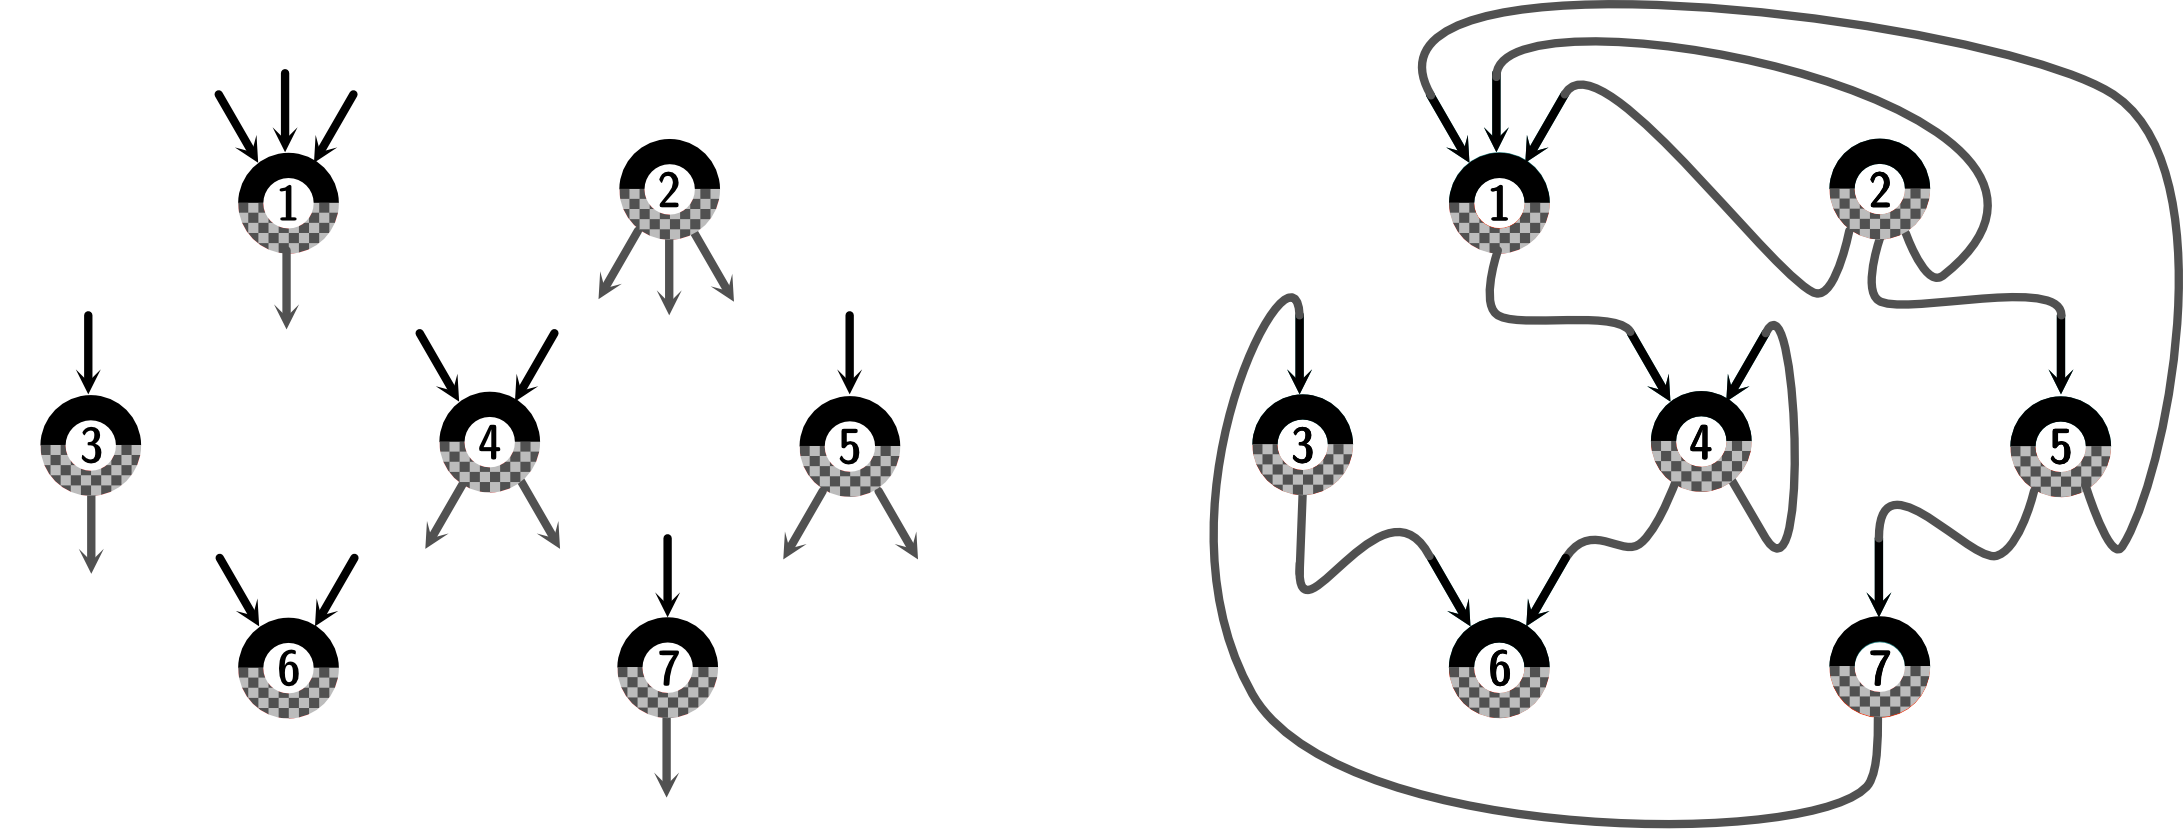
\includegraphics[width=0.90\textwidth]{ch2/fig/aap-figure_application.png}
    \caption{The DCM on $N=7$ vertices. The right panel shows a possible outcome for the matching.}
    \label{fig:illustration_singletype_DCM}
\end{figure}
Note that $\mathcal{G}_N$ may have loops and multi-edges, and also
vertices may have infinite total degrees. However, we are interested
in the lengths of directed paths in this graph: from any focal vertex
$i\in \{ 1,\ldots, N\}$ and for any fixed radius $r\geq 1$, there are only finitely
many paths (succession of directed edges) of total length less than
$r$ in $\mathcal{G}_N$.

Recall that the directed paths in the graph $\mathcal{G}_N$ model the
potential infections that may occur in a non-Markovian, discrete-time
epidemic with heterogeneous susceptibilities in the population. The
length of an edge $i\to j$ is the time needed after the infection of
$i$ for $j$ to become infected as a result of a contact with $i$. We
are typically interested in how the infection spreads from a focal
initially infected vertex, or conversely how it may reach this focal
vertex from potential sources of infection. By exchangeability, we use the vertex
indexed by $1$ as the focal vertex. Writing $\vec{d}(i,j)$ for the
minimal length of a directed path between two vertices $i$ and $j$, we
define, for $t\geq 1$,
\[
  \mathcal{V}_N(t) \ \coloneqq\ \big\{i\in \{ 1,\ldots, N\}:\ \vec{d}(1,i) \leq t\ \text{ or }\
  \vec{d}(i,1) \leq t\big\}
\]
the set of vertices that are at a directed distance of $1$ that is
less than $t$ in $\mathcal{G}_N$. We are interested in the rooted
decorated directed network $\mathcal{G}_N|_{t}$ whose vertex set is
$\mathcal{V}_N(t)$, with a root indexed by $1$, whose edge set is that
induced by $\mathcal{G}_N$, and where vertices are additionally
decorated with their total number of in- and outstubs of all types.
More precisely, we consider rooted decorated directed networks up to
isomorphism, \textit{i.e.} we forget about the labeling of vertices in
$\mathcal{G}_N|_{t}$. We refer to Figure~\ref{fig:exploration} for an
illustration of the part of $\mathcal{G}_N|_t$ accessible from the
root.
\begin{figure}[h]
    \centering
    \includegraphics[width=0.6\textwidth]{ch5/fig/aap-exploration.png}
    \caption{The out-exploration process of $\mathcal{G}$ from a
      source vertex. To find vertices at distance $n+1$ from the
      source, we traverse stubs with type $x$ that were added to the process at
      time $n-x+1$. The unmatched stubs in this picture are those going
      over the time horizon $n+1$, and those going backward from
      explored vertices.}
    \label{fig:exploration}
\end{figure}


We will be able to use Theorems~\ref{thm:ks_condition}
and~\ref{thm:type_convergence} to describe the distribution of
potential infectious contacts at time $t_N=\Theta(\log N)$ from the
focal vertex, as $N\to \infty$ and under some additional assumptions.
Among those, we impose the following moment conditions:
\begin{equation}\label{ch5_eq:moments}
  \mathbb{E}\big[(D^{\pm}_x)^2\big]\ <\ \infty,\qquad
  \mathbb{E}[D_x^-]\ =\ \mathbb{E}[D_x^+]\ =\ m_x, \qquad
  x\geq 1.
\end{equation}
In the following, we will let $\sigma_{x,\pm}^2$ denote the variance of
$D_x^{\pm}$.


\subsection{Main result} 

In order to motivate the study, we take one step ahead and state the main result of this work. Theorem~\ref{thm:geodesics} below holds under Assumption~\ref{ass:recurrence} and under \eqref{ch5_eq:moments} and~\eqref{eq:technical-condition-appli}. These assumptions give the existence and uniqueness of $\rho>0$ and non-negative random variables $W^{\pm}$ such that $\Prob(W^{\pm}>0)>0$. Let $\varnothing_-\in \{2,\ldots, N\}$ be a target vertex. We are interested in the sequence of directed path lengths going from a source $\varnothing_+\coloneqq 1$ to $\varnothing_-$ in  the graph $\mathcal{G}_N$. Denote  by $\mathcal{Q}_N$ this sequence, shifted by $\floor{\log_\rho(N)}$ and sorted in increasing order of discovery.

\begin{thm}[Convergence of directed path lengths]\label{thm:geodesics}
Under the previous assumptions, the sequence $(\mathcal{Q}_N)_N$ is tight: along every subsequence $N_j\to\infty$ such that $\floor{\log_\rho(N_j)}-\log_\rho(N_j)\to c\in[0,1]$, $\mathcal{Q}_{N_j}$ converges in distribution to a Cox point process $\mathcal{Q}_c$ indexed by $\Z$ and directed by
    \begin{equation*}
        \pi_c(T)= \rho^{T+c} W^+ W^-.
    \end{equation*}
% \jj{Il y aura quand même l'histoire de l'intensité du Cox multiplié par un terme qui dépend de $N$, mais du coup à voir comment formuler ça plus tard.
% Peut-être qu'une bonne manière de faire serait: la suite $...$ est tendue, et le long d'une sous-suite $(N_i)$ telle que $\floor{\log_\rho(N_j)}-\log_\rho(N_j)\to c$, on a la convergence en loi ...}
\end{thm}
As a consequence of Theorem~\ref{thm:geodesics}, we recover the following limit theorem for the distribution of the lengths of the first geodesics.
\begin{cor}\label{coro:distance_pairwise}
    In particular, denote by $(\vec{d}_N(i),i\leq k)$ the sequence giving the lengths to the $k\in\N$ shortest directed paths going from $\varnothing_+$ to $\varnothing_-$, shifted by $\floor{\log_\rho(N)}$. Then, $(\vec{d}_N(i),i\leq k)$ converges along every subsequence $N_j$ such that $\floor{\log_\rho(N_j)}-\log_\rho(N_j)\to c$ to the first $k$ atoms in $\mathcal{Q}$,
    \begin{equation*}
        \big(\vec{d}_{N_j}(i)-\floor{\log_\rho(N_j)}\big) \underset{N_j\to\infty}{\overset{(d)}{\longrightarrow}} (\pi_i, i\leq k).
    \end{equation*}
\end{cor}


\section{An algorithm to explore directed components}\label{sec:algo}
In the rest of this work, we explore the graph from multiple sources in order to recover the typical distances given in the main Theorem~\ref{thm:geodesics}.
In this section, we fix $\mathcal{G}_N$ to be a directed graph on $\{ 1,\ldots, N\}$ with integer edge lengths and two distinguished vertices $\varnothing^+$ and $\varnothing^-$, respectively called source and target. In addition, we fix an arbitrary labelling of the directed stubs -- which there is a countable number of. In the next sections, this graph will be a realization of the random DCM described in the previous section, but the algorithm presented in the current section is deterministic and can be applied to any graph.
To recover the directed loop-free paths joining two distinguished focal vertices, we explore the out-connected component of $\varnothing^+$ and the in-connected component of $\varnothing^-$ through a breadth-first-like exploration and record the forward paths.

We begin by giving heuristics for the exploration algorithm in order to motivate the reader, then the algorithm will be explained in detail in Section~\ref{sec:algo}.
\subsection{Heuristics}
Here we describe the exploration of the connected components graph forward from the source individual and backward to the target individual and identify the directed paths connecting one exploration to the other, as well as their lengths. To recover the paths with minimal lengths, we explore as in Section~\ref{ch2_sec:applications} of Chapter~\ref{chp2_ks_countable} in a breadth-first manner, but add a modification which ensures that the paths are discovered by increasing value of their length.


Each round of the directed explorations is split into two separate phases: a \textit{path-finding phase} followed by an \textit{exploration phase}.
\begin{itemize}
    \item In the \textbf{path-finding phase}, we reveal \textit{all} the possible paths connecting the source to the target vertices which have a given length -- that is during the path-finding stage of round $t$, we collect all the paths in the graph with length $2t-1$ or $2t$ connecting  $\varnothing^+$ to  $\varnothing^-$.
    \item In the \textbf{exploration phase}, the stubs located at the boundary of the connected components are traversed, expanding the connected components in both directions.
\end{itemize}
Both phases are done when exploring forward and backward, making each round consists in four stages.
Since we cannot explore the connected components simultaneously in the forward and backward directions, each phase of the algorithm must be further subdivided into a sequence of substeps. Each substep is defined conditionally on the filtration generated up to the immediately preceding substep. A substep corresponds to a single action involving either a pair of stubs (during a path-finding phase) or a single stub (during an exploration phase). Consequently, the arbitrary ordering of the stubs induces a corresponding ordering of the substeps.

We arbitrarily choose to alternate between the forward and backward directions by executing one step of the forward path-finding and exploration phases, followed by one step of the corresponding backward phases. Within each phase, the prescribed actions are carried out according to the induced ordering of the substeps.


\begin{rem}
The intuitive way of doing a breadth-first exploration follows up from the classical ``fluid mechanics'' metaphor of FPP from \cite{howard_models_2004}. In a nutshell, it consists in picturing the exploration as the progression of two fluids injected at $t=0$ into the source vertex and expanding at speed $1$ along the outward paths, and likewise backwards. The length of a directed path amounts to the time it takes the fluid to percolate from $\varnothing^+$ to $\varnothing^-$ along the edges of this path.
Following this naive algorithm, the stubs attached to vertices that are located one unit of length further away from the starting focal node are being traversed only after the traversal of every stub from vertices located closer to the focal ones. As a consequence, the sequence of path lengths is not monotonous: anticipating on the main result, for each point of the limit Cox process giving the length of the successively paths between $\varnothing^+$ and $\varnothing^-$, one would need to add a stochastic correction corresponding to the length of the connected edge to get the length of the path.
In the DCM, the correction can be shown to be geometrically distributed in the large $N$ limit, and the length and step of appearance of the geodesic is not a continuous function for the topology we will use to prove convergence of the point process $\mathcal{Q}_N$ introduced in Theorem~\ref{thm:geodesics}. 
\end{rem}

\subsection{Setting the framework}
% The formal description of the algorithm requires some further definitions and notations which we introduce here. 
% \begin{defn}[Generation of a stub]\label{def:generation_maturity}
%     The \textit{generation} $g(e)$ of a stub $e$ is defined as the round of the algorithm at which $e$ was reported by the exploration algorithm.
% \end{defn}

% \begin{defn}[Age and maturity]
%  The \textit{age} of a stub $e$ at round $t>g(e)$ corresponds to $a(t) \coloneqq  t-g(e).$
%     Thus, we will say that this stub becomes \textit{mature} when their age equals their length $x$, that is at round 
%    \[
%    t\ =\ g(e)+x.
%    \]
% \end{defn}
% We keep in mind that the notions of generation, age and maturity of a given stub depend on the algorithm.
As explained in the previous section, every round of the algorithm is subdivided into a finite (yet large) number of intermediate substeps. We will label the successive substeps of round $t\geq 0$ by 
\[
(t,k), \quad k\geq 0,
\]
using the convention that we identify $t$ with $(t,0)$ the substep just before starting round $t$.
We remind the reader that each round consists in four distinct stages:  forward path-finding, forward exploration, backward path-finding and backward exploration. As a consequence, the substeps $\big(t,k\big)_{k\geq 0}$ do not play the same role, but within the context of our work, this information is not relevant to be specified in the notations and we will simply use the latter notations to describe the substeps, keeping in mind that there is a finite number of them. 

Take a round $t\geq 0$ of the algorithm and assume we ran the algorithm up to the $k$-th substep of $t$. We denote by $\mathcal{E}^{+}(t,k)$ the set of outstubs who belong to the out-connected component of the source but have not yet been traversed just before substep $(t,k)$. More specifically, let $\mathcal{E}_{x,a}^+$ be the subset of $\mathcal{E}^{+}$ made by those having length $x$ and age $a$. 
We will use the notations $E^{+}_{N},\ E^{+}_{x,a}$ for the vector of number of such outstubs. Likewise we denote by $\mathcal{E}^{-}$ and $E^{-}$ the set of instubs and its cardinal.

Consider the row vectors $E^\pm(t,k)=  \big(E_{x,a}^\pm(t,k),\ (x,a)\in\mathcal{X}\big),$ where we recall Chapter~\ref{chp2_ks_countable} that 
$\mathcal{X}\ =\ \big\{(x,a)\in \N\times\N,\,a\leq x\big\}.$ We can now introduce the directed exploration processes. 
Identifying $t$ with $t_0$, the directed exploration processes defined by \begin{equation}\label{eq:exploration_process}\big(E^+(t),\ E^-(t)\big)\in \N^{\mathcal{X}*}\times \N^{\mathcal{X}*},\quad t\geq 0\end{equation} can be seen as a population process in which the individuals are the outstubs who either ``age'' (are replaced at $t+1$ by an individual with same length and age by one unit) or ``reproduce'' upon traversal (replaced by a multitype ``progeny'' corresponding to the collection of outstubs attached to the end node and who are still unseen). 
%  Particular importance will be attached to mature edges in the process, therefore to ease the notations we will use $\underline{Z}_N^{\square}$ for the restriction of the exploration processes to the mature edges. 
%  Put differently for $x,t\in\N$ we have

% \begin{equation*}
%     \underline{Z}_{N,x}^{\mt}(t) \ \coloneqq\  Z_{N,(x,x)}^{\square}(t).
% \end{equation*}
% Throughout this work we will use the convention to ``underline'' quantities for the canonical reduction to mature types.
We also keep track of {$\mathcal{I}^{\pm}(t,k)$} the set of nodes that have been discovered through the $\pm$-exploration up to substep $(t,k)$, which we will call infected vertices. For instance, vertex labelled $i$ belongs to the set $\mathcal{I}^{+}(t,k)$ if and only if at substep $(t,k)$, we reported the outstubs going out of $i$. Finally, for every $i\in\{ 1,\ldots, N\}$ we denote by 

\[I_i^\pm(t,k)\ \coloneqq\ \1\big(i\in \mathcal{I}^\pm(t,k)\big)\]
the two variables encoding the forward/backward infection status of vertex labelled $i$.


\subsection{The path-finding and exploration phases}
In this section we fix a step $t$ of the algorithm and consider only the forward exploration, the backward situation being analogous. We refer to Firgure~\ref{fig:path_finding} for an illustration of this so-colled path-finding phase.
\paragraph{Revealing the paths.}
 We allow the matching of non-mature yet stubs, however every stub have to be matched (that is, die in the population process) by the time they reach maturity, guaranteeing the absence of stubs having age greater than their length.

Step $t$ of the out-exploration reveals \emph{all paths} with length $2t-1$. These paths are composed from edges with length $x\leq 2t-1$.

Let $x\in\{ 1,\ldots 2t-1 \}$. We introduce ${G_x(t)}$ the set of integers satisfying
    \begin{equation}\label{eq:set_G_xt}
        \begin{aligned}
          \text{if }  x\leq t,&\quad  G_{x}(t)\ \coloneqq\ \{ t-x, \ldots, t-1 \}, \text{ such that }\abs[\big]{G_{x}(t)}= x,\\
             \text{if }  x\geq t+1 ,&\quad G_{x}(t)\ \coloneqq\ \{ 0,\ldots, 2t-x \},\text{ such that } \abs[\big]{G_{x}(t)}= 2t-x.
        \end{aligned}
    \end{equation}
For $x \in \{1,\ldots,2t-1\}$ and $g\in G_x(t)$, denote by $g'\in\{ 0,\ldots, t-1 \}$  such that 
\[
g+g'+x \ =\ 2t-1.
\]
Let $(e_1,e_2,\dots)$ and $(e'_1,e'_2,\dots)$ be the induced ordering of the finite sets $\mathcal{E}^+_{x,t-g}(t)$ and $\mathcal{E}^-_{x,t-g'}(t)$.
 Then in increasing order of $i$ and $j$, we test the potential connection of $e_i$ and $e'_j$. On the event that this corresponds to substep $(t,k)$, two situations can happen:
 \begin{itemize}
    \item Either this connection is present in the graph. In this case, a path connecting the source to the target vertices has been found by the exploration. Note that by construction, the length of this path equals $g+g'+x = 2t-1$. In this case, we remove both stubs from the pool of ``free'' stubs. That is $e_i\notin \mathcal{E}^+(t, k+1)$ and  $e_i\notin \mathcal{E}^-(t, k+1)$. 
    \item  Or the matching is unsuccessful. In this case we do not know yet the end vertex of these stubs. They are left untouched and remain in the exploration processes as candidate for matching in future rounds of the algorithm, until they reach maturity.
 \end{itemize}
 

 \begin{figure}[H]
    \centering
  \resizebox{0.95\textwidth}{!}{ 
      \begin{tikzpicture}[x=0.75pt,y=0.75pt,yscale=-1,xscale=1]
        %uncomment if require: \path (0,434); %set diagram left start at 0, and has height of 434
        
        %Image [id:dp3360541416240077] 
        \draw (487,212.39) node  {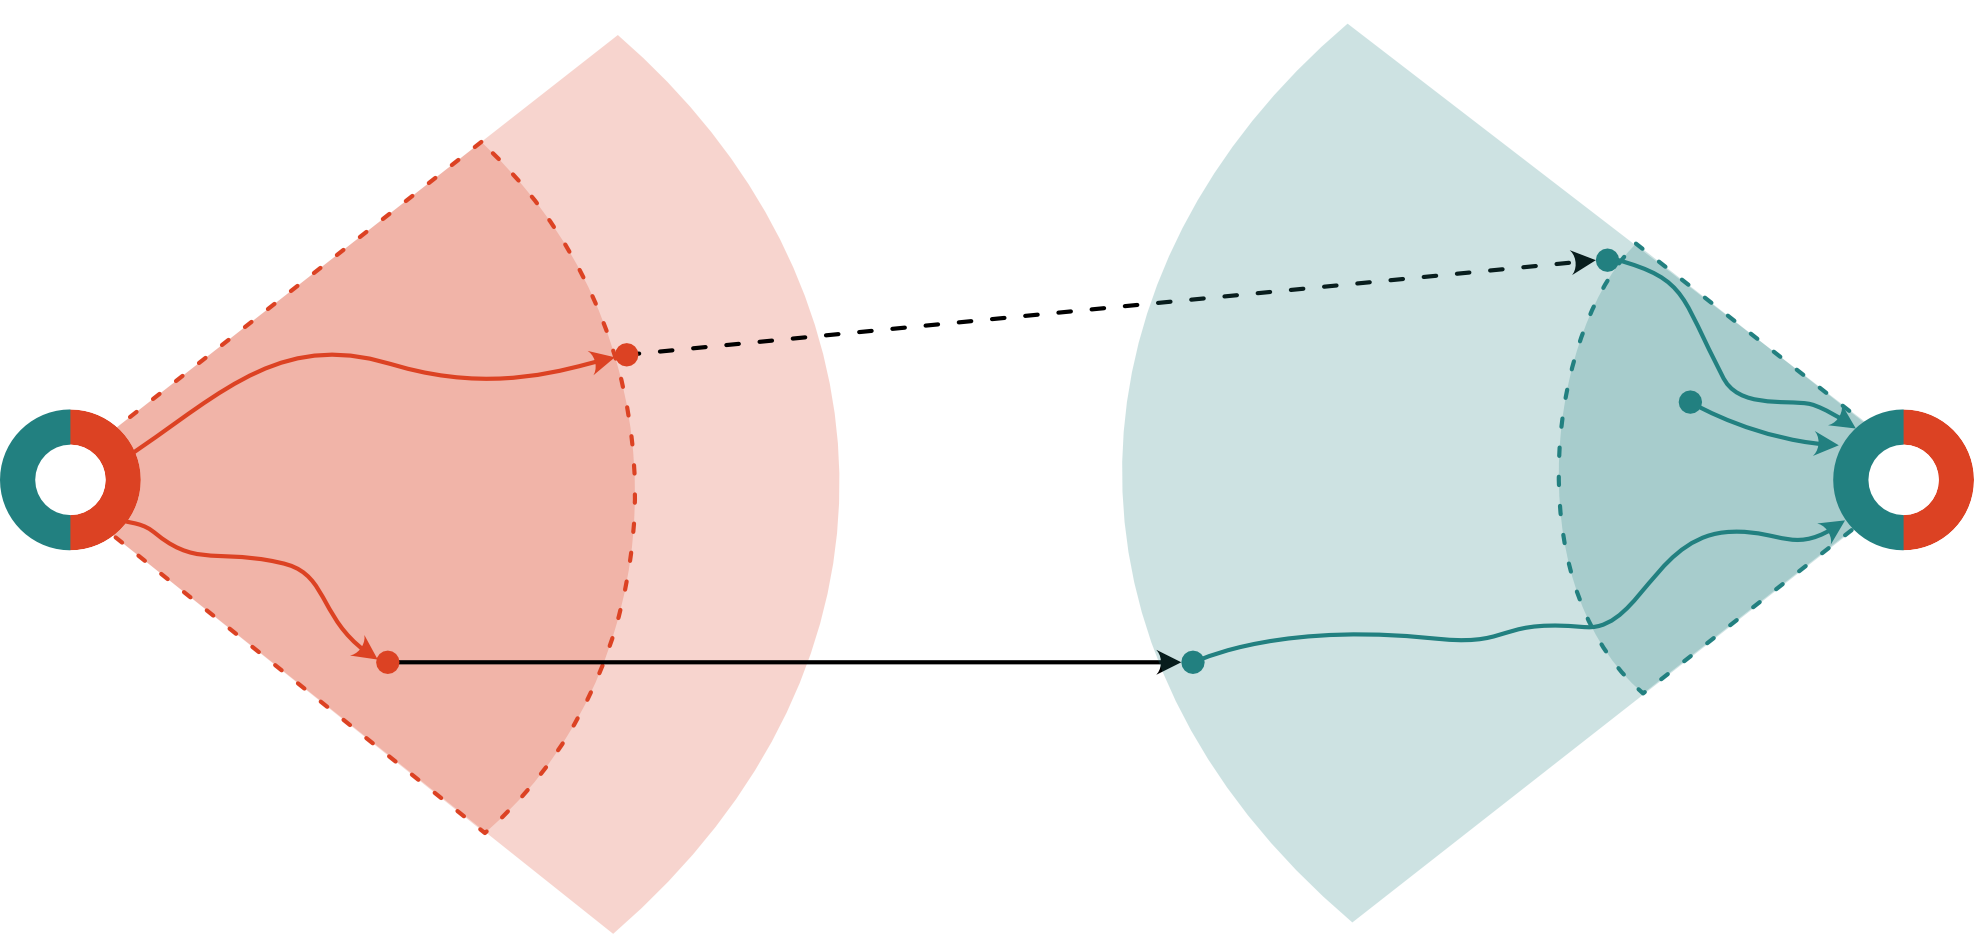
\includegraphics[width=711pt,height=338.25pt]{ch5/fig/path_finding.png}};
        
        % Text Node
        \draw (255,110) node [anchor=north west][inner sep=0.75pt]  [font=\LARGE]  {$e_i\in \mathcal{E}^+_{ x ,t-g }(t,k)$};
        % Text Node
        \draw (30,204) node [anchor=north west][inner sep=0.75pt]  [font=\LARGE]  {$\varnothing^{+}$};
        % Text Node
        \draw (127,315) node [anchor=north west][inner sep=0.75pt]  [font=\LARGE]  {$\begin{array}{l} \tilde{e}\notin\mathcal{E}^+(t,k)\\\textit{removed from the process} \end{array}$};
        % Text Node
        \draw (910,204) node [anchor=north west][inner sep=0.75pt]  [font=\LARGE]  {$\varnothing^{-}$};
        % Text Node
        \draw (679,40) node [anchor=north west][inner sep=0.75pt]  [font=\LARGE]  {$ \begin{array}{l}
        e'_j\in \mathcal{E}^-_{ x ,t-g' }(t,k)
        \end{array}$};
        % Text Node
        \draw (560,321) node [anchor=north west][inner sep=0.75pt]  [font=\LARGE]  {$\tilde{e}',\ g(\tilde e')=t-1$};
        % Text Node
        \draw (540,170) node [anchor=north west][inner sep=0.75pt]  [font=\LARGE]  {$e'_{j'}\in \mathcal{E}^-_{x ,t-g'' }(t,k),\ g''< g'$};
        % Text Node
        \draw (472,107) node [anchor=north west][inner sep=0.75pt]  [font=\LARGE]  {$?$};
        % Text Node
        \draw (466,274) node [anchor=north west][inner sep=0.75pt]  [font=\LARGE]  {$\checkmark $};
        \draw (700,350) node [anchor=north west][inner sep=0.75pt]  [font=\LARGE]  {
          \textit{free instubs
          not connected to $e_i$}};
          % Text Node
\draw (10,60) node [anchor=north west][inner sep=0.75pt]  [font=\LARGE]  {  \textit{free outstubs
          not connected to $e'_j$}};

          %Curve Lines [id:da7296032106762098] 
\draw [line width=1.5]    (869.25,335.8) .. controls (867.31,312.52) and (811.5,312.48) .. (826.41,274.17) ;
\draw [shift={(828,270.5)}, rotate = 115.46] [fill={rgb, 255:red, 0; green, 0; blue, 0 }  ][line width=0.08]  [draw opacity=0] (13.4,-6.43) -- (0,0) -- (13.4,6.44) -- (8.9,0) -- cycle    ;
%Curve Lines [id:da6919472054664801] 
\draw [line width=1.5]    (77,99.5) .. controls (80.92,147.52) and (124.22,119.67) .. (180.54,130.77) ;
\draw [shift={(184,131.5)}, rotate = 192.63] [fill={rgb, 255:red, 0; green, 0; blue, 0 }  ][line width=0.08]  [draw opacity=0] (13.4,-6.43) -- (0,0) -- (13.4,6.44) -- (8.9,0) -- cycle    ;
        
        
        \end{tikzpicture}
    }
        \caption{Illustration of a substep $(t,k)$ in the forward path-finding phase of round $t$ of the algorithm. This substep consists in testing the connection between $e_i\in \mathcal{E}_{x,t-g'}^-(t,k)$ and $e'_j\in \mathcal{E}_{x,t-g'}^-(t,k)$ where $  g' =2t-1-g -x$. A previous step of the algorithm revealed the connection $\tilde{e}\to \tilde{e}'$, removing them from the pool of free stubs at $(t,k)$. The instub $e'_{j'}$ have length $x$ and is unmatched at $(k,t)$ but the connection $e_i\to e'_{j'}$ would a path with length $>2t-1$, hence it will be tested in a further round of the algorithm if neither $e_i$ nor $e'_{j'}$ are matched before.}
    \label{fig:path_finding}
\end{figure}

\paragraph{Expanding the connected components.}
 In the (forward) exploration phase, we traverse the mature outstubs that are still in the exploration processes to reveal the instub they instub it is connected to. Since the possibilities of creating a path through this stubs have already been tested, the connecting outstub is not in the backward exploration process at the current substep. This way, we expand the connected components in the directions of mature stubs. We refer to Figure~\ref{fig:exploring} for an illustration of the exploration phase.

 \begin{figure}[H]
 \centering
    \resizebox{0.75\textwidth}{!}{  


  \begin{tikzpicture}[x=0.75pt,y=0.75pt,yscale=-1,xscale=1]
  %uncomment if require: \path (0,475); %set diagram left start at 0, and has height of 475
  
  %Image [id:dp1370742743197475] 
  \draw (262.58,239.74) node  {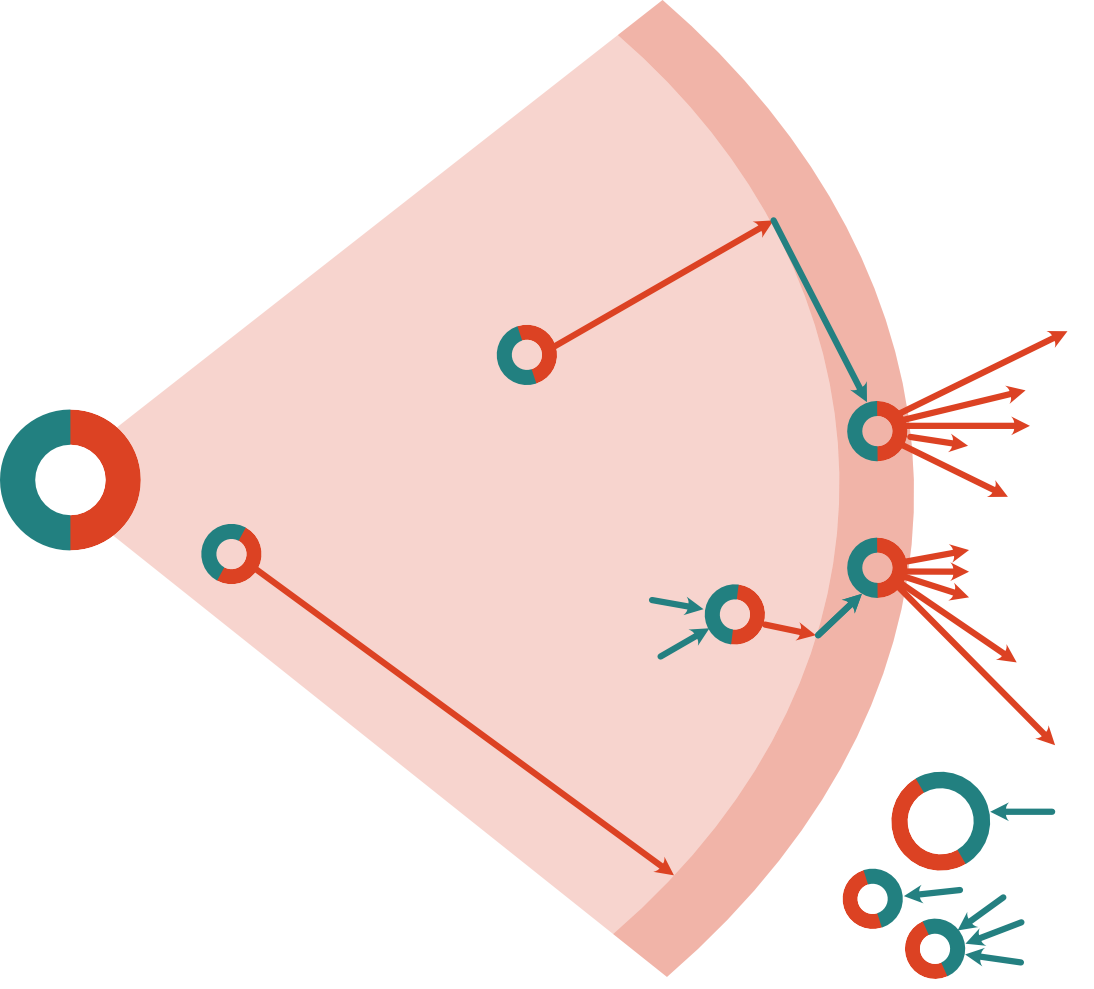
\includegraphics[width=390.87pt,height=351.23pt]{ch5/fig/exploration_phase.png}};
  %Shape: Brace [id:dp4771671339342859] 
  \draw  [line width=1.5]  (402.12,197.58) .. controls (397.45,197.65) and (395.15,200.01) .. (395.22,204.68) -- (395.57,230.47) .. controls (395.66,237.14) and (393.38,240.5) .. (388.71,240.56) .. controls (393.38,240.5) and (395.76,243.8) .. (395.85,250.46)(395.81,247.46) -- (396.23,278.26) .. controls (396.3,282.93) and (398.66,285.23) .. (403.33,285.17) ;
  %Shape: Brace [id:dp5554713219615801] 
  \draw  [line width=1.5]  (502.57,367.38) .. controls (507.24,367.45) and (509.6,365.16) .. (509.67,360.49) -- (511.04,269.47) .. controls (511.14,262.8) and (513.52,259.5) .. (518.19,259.57) .. controls (513.52,259.5) and (511.24,256.14) .. (511.34,249.47)(511.29,252.47) -- (512.66,161.05) .. controls (512.73,156.39) and (510.44,154.02) .. (505.77,153.95) ;
  %Shape: Brace [id:dp9378467695242451] 
  \draw  [line width=1.5]  (506.79,469.95) .. controls (511.46,469.84) and (513.73,467.45) .. (513.62,462.78) -- (512.46,415.06) .. controls (512.3,408.39) and (514.55,405) .. (519.21,404.89) .. controls (514.55,405) and (512.14,401.73) .. (511.97,395.06)(512.05,398.06) -- (511.73,385.21) .. controls (511.62,380.54) and (509.23,378.27) .. (504.57,378.38) ;
  
  % Text Node
  \draw (20,221) node [anchor=north west][inner sep=0.75pt]  [font=\LARGE]  {$\varnothing^{+}$};
  % Text Node
  \draw (200,227) node [anchor=north west][inner sep=0.75pt]  [font=\LARGE]  {$\in \mathcal{I}^{+}(t,k) \setminus \mathcal{I}^{+}( t,0)$};
  % Text Node
  \draw (190,80) node [anchor=north west][inner sep=0.75pt]  [font=\LARGE]  {$e\in \underline{\mathcal{Z}}_{N}^{+}( t,k-1)$\textit{ traversed at }$(t,k)$};
  % Text Node
  \draw (525,245) node [anchor=north west][inner sep=0.75pt]  [font=\LARGE]  {\textit{outstubs in }$\mathcal{Z}_{N}^{+}( t,k)$};
  % Text Node
  \draw (360,310) node [anchor=north west][inner sep=0.75pt]  [font=\LARGE]  {$e'$};
  % Text Node
  \draw (0,350) node [anchor=north west][inner sep=0.75pt]  [font=\LARGE]  {\textit{mature stub to be}};
 \draw (0,380) node [anchor=north west][inner sep=0.75pt]  [font=\LARGE]  {\textit{traversed in} $(t,k'),\ k'>k$};
  % Text Node
  \draw (30,150) node [anchor=north west][inner sep=0.75pt]  [font=\LARGE]  {\textit{vertex in} $ \mathcal{I}^{+}(t,k-1)$};
  % Text Node
  \draw (525,389) node [anchor=north west][inner sep=0.75pt]  [font=\LARGE]  {\textit{instubs not in }$\mathcal{Z}_{N}^{-}( t,k)$};
  % Text Node
  \draw (443,383) node [anchor=north west][inner sep=0.75pt]  [font=\LARGE]  {$\bm{\dagger} $};
  
  
  \end{tikzpicture}
  }
  \caption{Illustration of the exploration phase of the algorithm. The mature outstubs at round $t$ reach the ``boundary'' of the exploration, pictured in a darker shade of red. Here we assume that substep $(t,k)$ corresponds to traversing the mature outstub $e\in \mathcal{E}^+(t,k-1)$ and revealing the connection to a vertex. In this realization, the vertex $N_e$ to which $e$ leads was not infected at $(t,k-1)$. Hence at step $k$, we set $I^+_{N_e}(t,k)=1$ and add the collection of ousttubs $D_{N_e}^+$ to $\mathcal{E}^+(t,k)$. The vertex $N_e$ is at distance $t$ from the source $\varnothing^+$. The mature outstub $e'$ was traversed at a previous substep of the exploration phase of round $t$, hence is removed from the process. The pool of free instubs remaining to be matched is picture in green.}
       \label{fig:exploring}
\end{figure}

\subsection{Markovian exploration of the DCM}

To conclude this section, we apply the exploration algorithm to the random directed configuration model with edge lengths  on $\{ 1,\ldots, N\}\cup \dagger$ presented in Section~\ref{sec:model}. This section aims to derive the probability to recover paths connecting $\varnothing^-$ to $\varnothing^+$ having a given length. Each substep of the algorithm reveals information on the connections present in the DCM. Hence for $t\geq 0$ and $k\geq 1$, we denote by $\mathcal{F}_N(t,k)$ the canonical $\sigma$-field $\mathcal{F}_N(t,k)$ containing all the information up to substep $(t,k)$ of the exploration algorithm. As before, we use the convention that for $t\geq 1$, substep $t=(t,0)$ corresponds to the last substep of round $t-1$, in such a way that

\begin{align*}
\forall t\geq 1,\ \mathcal{F}_N(t)\ &\coloneqq \bigvee_{k\geq 1} \mathcal{F}_N(t-1,k)\ = \ \sigma\Big(\bigcup_{k\geq 1} \mathcal{F}_N(t-1,k)\Big),\\
\mathcal{F}_N(0)\ &= \sigma(\emptyset).
\end{align*}



The algorithm is designed so that each pair of non-mature half-edges and every mature stub is looked at only once, thus at every substep $(t,k)$ the processes $E^{\pm}(t,k)$ and $\mathcal{I}^{\pm}(t,k)$ are Markov processes adapted to $\mathcal{F}_N(t,k)$.  In particular, we stress that every substep in the path-finding phase test does not reveal the end-node of a directed stub, but only test whether a connection exists between two given stubs.




Fix $t\geq 1$. According to the algorithm, the paths connecting the source to the target which length $2t-1$ or $2t$ can only be discovered during round $t$, and we recover all of them. As before, everything being symmetric we only describe the forward situation, which corresponds to paths with odd length (here, $2t-1$).
Assume the graph has been explored up to round $t-1$ of the previously described algorithm. 
Revealing a connection that create path with length $2t-1$ is a binary test which amounts to tossing an independent coin. Let $x\geq 1$ and recall the set $G_x(t)$ from \eqref{eq:set_G_xt}, $g'$ such that $g+g'+x = 2t-1$ and the ordering of stubs used previously.

\begin{prop} \label{prop:exploration_process_is_good}
 Let $k\geq 1$ and $g, g', x$ be such that $g+g'+x=2t-1$.  
 Then conditional upon $\mathcal{F}_N(t,k-1)$ and on the event that substep $(t,k)$ corresponds to testing the connection between $e_i\in \mathcal{E}_{x,t-g}^+(t,k-1)$ and $e'_j\in \mathcal{E}_{x,t-g'}^-(t,k-1)$, the probability to observe a successful matching  is a given by $p(t,k)$, satisfying
 \begin{multline}\label{eq:path_probability_p_txg}
      \frac{1}{p(t,k)}\  = \ K_{N,x}(t,k)\ - \sum_{g''<g}E_{x,t-g''}^+(t,k-1) - \sum_{g''<g'}E_{x,t-g''}^-(t,k)\\
- (i-1) - (j-1) + 2\sum_{i'< i}\sum_{j'< j} \1(e_{i'}\to e'_{j'}),
\end{multline}
where $2K_{N,x}(t,k)$ is the number of unmatched $x$-type stubs just before the current substep. By construction of the algorithm, $p(t,k)$ is the probability of finding a path $\varnothing^+\to\varnothing^-$ with length $2t-1$ at substep $(t,k)$.
\end{prop}
The proof of Proposition~\ref{prop:exploration_process_is_good} is deferred to Appendix~\ref{sec:matching_bipartite}.
 

\section{Geodesics in the DCM with edge lengths}\label{sec:paths}

This section is dedicated to the proof of the main theorem of this work, which gives the weak convergence of the lengths of the directed paths from $1$ to $u$ shifted by $2T_N$ towards the atoms of a point process whose intensity is explicitly expressed as a function of the system parameters. Let $T=o(\log N)\in \Z$. The results of Section~\ref{ch2_sec:applications} in Chapter~\ref{chp2_ks_countable} ensure that the number of half-edges that can make a path with length $2T_N+T$ is close to the size of the branching processes, with high probability as $N\to\infty$.

\subsection{Topology for some discrete point processes}
First and foremost we need to define a topology for the convergence of point processes in $\Z$. 
\begin{defn}[Topology $\mathscr{T}$]\label{def:weak_topology}
  Let $\mathcal{X}$ be a countable set and let $\mathcal{M}=\mathcal{M}_{\mathcal{X}}$ be the set of point measures $\mu$ on $\Z\times \mathcal{X}$ such that $\mu((-\infty,k]\times \mathcal{X})<\infty$ for all $k\in \mathbb{Z}$.
  We think of $\mathcal{X}$ as a set of discrete \emph{types} that serve as marks on the point process $\mu$.
  
  We endow $\mathcal{M}$ with the topology $\mathscr{T}$ such that a basis of open sets is composed of sets of the form
  \[
    \big\{\mu \in \mathcal{M} : \mu_{|(-\infty,k]\times \mathcal{X}} = \nu \big\},
  \]
  for $\nu$ a finite point measure on $(-\infty,k]\times \mathcal{X}$.
  Since this basis is countable, $\mathscr{T}$ is separable.
  Furthermore, note that $\mathscr{T}$ is metrizable, for instance thanks to the metric:
  \[
    d_{\mathscr{T}}(\mu, \mu')\ =\ \mathrm{exp}\Big(-\sup\{k\in \mathbb{Z} : \mu_{|(-\infty,k]\times \mathcal{X}} = \mu'_{|(-\infty,k]\times \mathcal{X}}\}\Big).
  \]
  We will say that $\mu$ and $\mu'$ \emph{agree up to $k$} if $\mu_{|(-\infty,k]\times \mathcal{X}} = \mu'_{|(-\infty,k]\times \mathcal{X}}$.
\end{defn}

\begin{rem} \label{rem:continuity_first_point}
  Note that with this definition, it is not difficult to see that the ``first-point'' map $\mu\in \mathcal{M}\mapsto \inf \{k :  \mu((-\infty,k]\times \mathcal{X}) \neq 0\}$ is continuous.
  This can easily be extended to keep track of the types $\mathcal{X}$, and to cover the $n$ first points.
\end{rem}

The idea is to record the substeps in the exploration algorithm at which paths are found between the focal vertices.

\subsection{Poisson approximation in $\mathcal{M}_{\mathcal{X}}$}
Here, we give bounds between a Bernoulli-type model of point process $\mathcal{N}$ in $\mathcal{M}$ and its Poissonized version $\widehat{\mathcal{N}}$ (which is actually a Cox process since we will allow its intensity to be random).
Let us be more specific to describe the setting we work with.
We consider a random point process $\mathcal{N}$ valued in $\mathcal{M}$ built by setting
\[
  \mathcal{N}\ =\ \sum_{(k,x)\in \mathbb{Z}\times \mathcal{X}} \bigg(\sum_{\ell \geq 1} X_{k,\ell}^x \bigg)\delta_{k,x},
\]
where the $(X_{k,\ell}^x)$ are Bernoulli random variables.
Assume that:
\begin{itemize}
  \item There are $\sigma$-fields $(\mathcal{F}_{k,\ell}^x, (k,\ell,x)\in \mathbb{Z}\times \mathbb{N} \times \mathcal{X})$, and $\mathcal{F}_k = \bigvee_{x,\ell}\mathcal{F}_{k,\ell}^x$. Each random variable $X_{k,\ell}^x$ is $\mathcal{F}_{k,\ell}^x$-measurable.
  \item There is a fixed numbering of $\mathcal{X}$ (\ie a bijection with $\mathbb{N}$), inducing a well-founded total order on it.
  Let us write $x_1$ as its minimum element.
  \item $(\mathcal{F}_{k,\ell}^x)$ is a filtration for the lexicographic order on $(k,x,\ell)\in \mathbb{Z}\times \mathcal{X}\times \mathbb{N}$; in other words, we have $\mathcal{F}_{k,\ell-1}^x\subset \mathcal{F}_{k,\ell}^x$, where in the case $\ell=1$, we further define
  \[
    \mathcal{F}_{k,0}^x\ =\ \begin{cases}
      \bigvee_{\ell}\mathcal{F}_{k,\ell}^{x_i} &\text{if }x=x_{i+1}, i\in \mathbb{N},\\
      \mathcal{F}_{k-1} &\text{if }x=x_1.
    \end{cases}
  \]
\end{itemize}
For the moment, note that the existence of such a filtration does not hold meaning in itself: given the $(X_{k,\ell}^x)$ one can always consider the  natural filtration.

\begin{lem} \label{lem:poisson_approximation}
  With the definitions and notation as above, we write
  \[
    p_{k,\ell}^x = \mathbb{P}\Big(X_{k,\ell}^x = 1 \mid \mathcal{F}_{k,\ell-1}^x\Big).
  \]
  Assume that there exists $k_0\in \mathbb{Z}$ and some nonnegative random variables $(\pi_{k,\ell}^x, k\geq k_0+1,\ell\geq 1,x\in \mathcal{X})$ such
  that $\pi_{k,\ell}^x$ is $\mathcal{F}_{k_0}$-measurable, and we define $\pi_{k}^x = \sum_{\ell}\pi_{k,\ell}^x$.
%  that $\pi_{k,\ell}^x$ is $\mathcal{F}_{k}$-measurable, and for each fixed $k$, conditional on $\mathcal{F}_{k-1}$, we have
%  \[
%  (\pi_{k,\ell}^x)_{\ell,x} \indep (p_{k,\ell}^x)_{\ell,x}
%  \]
  Then we can build, on the same probability space, a Cox process $\widehat{\mathcal{N}}$ on $\mathbb{Z}\times \mathcal{X}$, directed by $\pi_{k}^x$, in such a way that for all $k_1>k_0$,
  \begin{multline*}
    \mathbb{P}\Big(\mathcal{N}\text{ and } \widehat{\mathcal{N}}\text{ agree up to }k_1\Big) \geq 1  - C_1 \mathbb{E}\bigg[\sum_{k=k_0+1}^{k_1}\sum_{x,\ell}\Big( (p_{k,\ell}^x)^2 + (\pi_{k,\ell}^x)^2 + |p_{k,\ell}^x - \pi_{k,\ell}^x|\Big)\bigg] \\
    - \mathbb{P}\Big(\mathcal{N}((-\infty,k_0]\times \mathcal{X})>0\Big),
  \end{multline*}
  where the constant $C_1$ is universal.
\end{lem}

\begin{proof}
  The key idea is an easy-to-show inequality for coupling Bernoulli and Poisson random variables: there exists a universal constant such that
  \[
  d_{\mathrm{TV}}\big(\mathrm{Be}(p),\mathrm{Poi}(\pi)\big) \leq C_1 \big(p^2+\pi^2+\abs{p-\pi}\big).
  \]
  Indeed,
  \begin{equation*}
    d_{\mathrm{TV}}\big(\mathrm{Be}(p),\mathrm{Poi}(\pi)\big) =\frac{1}{2}\big(\abs{1-p-\e^{-\pi}}+\abs{p-\pi\e^{-\pi}}+\Prob\big(\mathrm{Poi}(\pi)\geq 2\big)\big)
  \end{equation*}
For $\pi\geq$ or $p\geq 1$, we can crudely bound the total variation by 1.
A Taylor expansion and Markov's inequality leads to the conclusion for small $\pi,p<1$.
\begin{align*}
    d_{\mathrm{TV}}\big(\mathrm{Be}(p),\mathrm{Poi}(\pi)\big) &\leq\frac{1}{2}\big( 2\abs{p-\pi}+O(\pi^2+p^2)+\pi^2\big)\\
    &\leq C_1 \big(p^2+\pi^2+\abs{p-\pi}\big).
  \end{align*}
 
  Up to enriching our probability space, we may assume that for each $k>k_0$ and $(\ell,x)\in \mathbb{N}\times \mathcal{X}$, we jointly draw $X_{k,\ell}^x$ and a new random variable $Y_{k,\ell}^x$ such that
  \begin{itemize}
    \item conditional on $\mathcal{F}_{k,\ell-1}^x$, $X_{k,\ell}^x\sim \mathrm{Be}(p_{k,\ell}^x)$ and $Y_{k,\ell}^x\sim \mathrm{Poi}(\pi_{k,\ell}^x)$.
    \item $\mathbb{P}(X_{k,\ell}^x\neq Y_{k,\ell}^x \mid \mathcal{F}_{k,\ell-1}^x) \leq C_1 ((p_{k,\ell}^x)^2+(\pi_{k,\ell}^x)^2+\lvert p_{k,\ell}^x-\pi_{k,\ell}^x\rvert )$.
    \item $Y_{k,\ell}^x$ is $\mathcal{F}_{k,\ell}^x$-measurable.
  \end{itemize}
  These new variables $(Y_{k,\ell}^x)$ are of course not independent of the $(X_{k,\ell}^x)$, but because the family $(\pi_{k,\ell}^x)$ is $\mathcal{F}_{k_0}$-measurable they form an independent family. Furthermore, conditional upon $\sigma((\pi_{k,\ell}^x))$, they are all Poisson distributed with respective parameter $\pi_{k,\ell}^x$.
  Therefore, the point process
  \[
    \widehat{\mathcal{N}}\ =\ \sum_{k,x} Y_{k}^x\delta_{k,x}, \quad \text{with} \quad Y_{k}^x = \sum_{\ell\geq 1} Y_{k,\ell}^x
  \]
  has indeed the right Cox process distribution.
  
  Now by construction, and with an easy induction, for any finite subset of indices $F\subset \mathbb{Z}\times \mathcal{X} \times \mathbb{N}$, we get
  \begin{align*}
    \mathbb{P}\bigg( \bigcap_{(k,x,\ell)\in F}\{X_{k,\ell}^x = Y_{k,\ell}^x \}\bigg)\ &\geq\ \mathbb{E}\bigg[\prod_{(k,x,\ell)\in F} \Big(1- C_1 ((p_{k,\ell}^x)^2+(\pi_{k,\ell}^x)^2+|p_{k,\ell}^x-\pi_{k,\ell}^x|)\Big)_+\bigg] \\
    &\geq\ \mathbb{E}\bigg[1-\Cte \sum_{(k,x,\ell)\in F} \Big((p_{k,\ell}^x)^2+(\pi_{k,\ell}^x)^2+|p_{k,\ell}^x-\pi_{k,\ell}^x|\Big)\bigg],
  \end{align*}
thus by monotone convergence (letting $F\uparrow [k_0+1,k_1]\times \mathcal{X}\times \mathbb{N}$) and because by construction $\widehat{\mathcal{N}}((-\infty,k_0]\times \mathcal{X})=0$, we obtain
\begin{multline*}
  \mathbb{P}(\mathcal{N}\text{ and } \widehat{\mathcal{N}}\text{ agree up to }k_1)\ \geq\ 1  - C_1 \mathbb{E}\bigg[\sum_{k=k_0+1}^{k_1}\sum_{v,\ell}\Big( (p_{k,\ell}^x)^2 + (\pi_{k,\ell}^x)^2 + |p_{k,\ell}^x - \pi_{k,\ell}^x|\Big)\bigg]\\
- \mathbb{P}\Big(\mathcal{N}\big((-\infty,k_0]\times \mathcal{X}\big)>0\Big),
\end{multline*}
concluding the proof.
\end{proof}


 \subsection{Proof of the main result}
 In the following, we shift lengths by a quantity $2T_N$. We call ``connecting stub'' the half-edge (whether they are in or out stubs) through which we discover a directed path connecting the out-connected component to the in-connected component of the exploration processes. From the algorithm presented in Section~\ref{sec:algo}, connecting stubs are revealed in the path-finding phase as a result of a Bernoulli coin tossing experiment, either by pairing an instub of $E^+$ to an element of $E^-$ or \textit{vice-versa}. Therefore, the successively discovered tuples consisting of the directed paths' lengths in the shifted frame and the length of the connecting stub define a Bernoulli-type point process with values in $\mathcal{M}$. We will denote this point process as $\mathcal{Q}_{N}$.  Recalling that for $T\geq - 2T_N,$ $t_N=\lfloor T_N+T/2\rfloor$, we have
 \begin{equation}\label{eq:path_point_process_bernoulli}
    \mathcal{Q}_{N}\ =\sum_{T\in \Z}\sum_{x\in  \N}\bigg[\sum_{g\in G_x(t_N)}\sum_{(i,j)\in \mathcal{S}^{B}_{(x,g)}}B\big({t_N}^\pm_{\textit{path}}(x,g,i,j)\big)\bigg]\delta_{T,x},
 \end{equation}
 where  $(\pm,\mp)=(+,-)$ when $T$ is odd, $(-,+)$ otherwise,
and for $T<-2T_N$ the intensity is set to zero.
The inner sum in \eqref{eq:path_point_process_bernoulli} is on pairs belonging to the subset of $\N^2$ defined as

\[\mathcal{S}^{B}_{(x,g)}=\big\{ (i,j)\in\N^2: i\leq \abs{E^\pm_{x,t_N-g}(t_N)},\,j\leq\abs{E^\mp_{x,t_N-g'}(t_N)}\Big\}.\] 
Let $T_0\in \Z$, $t_N^0=\lfloor T_N+T_0/2\rfloor$.  From Lemma~\ref{lem:poisson_approximation}, we can build a Cox process $\widehat{\mathcal{Q}}_{N}$ which is coupled with $\mathcal{Q}_N$. Conditional upon $\mathcal{F}(t_N^0)$, $\widehat{\mathcal{Q}}_{N}$ is distributed as a Poisson point process with intensity 
 $\mathcal{Q}_N$, and its intensity at $T\geq T_0$ is given by \eqref{eq:pi_N_cox_intensity}.
 
 \begin{align}\nonumber
    \pi_N^{(T,x)}&=\sum_{g\in G_x(t_N)}\sum_{(i,j)\in\mathcal{S}^P_{(x,g)}}\frac{1}{N m_x\vee 1}\\\label{eq:pi_N_cox_intensity}
    &=\rho^T W^+(t_N^0)W^-(t_N^0)\tilde{h}^+_{xx}\tilde{h}^-_{xx}\frac{x\rho^x}{m_x}\Big(1 \wedge Nm_x\Big),
\end{align}
the inner sum in the first line being on the subset of $\N^2$ defined as
\begin{equation}\label{eq:S^P_x_g}
  \mathcal{S}^{P}_{(x,g)}\ \coloneqq\ \big\{ (i,j)\in\N^2: i\leq W^{\pm}(t_N^0)\rho^{x+g}\tilde{h}^{\pm}_{xx},\,j\leq W^{\mp}(t_N^0)\rho^{x+g'}\tilde{h}^{\mp}_{xx}\Big\},
\end{equation}
  whence \eqref{eq:pi_N_cox_intensity}.
Applying Lemma~\ref{lem:poisson_approximation}, for $T_0<T_1\in \Z$ we have
\begin{align}\nonumber
  \Prob\big(\mathcal{Q}_{N} \text{ and }\widehat{\mathcal{Q}}_{N} & \begin{multlined}[t]\text{ agree up to }T_1\big)
    \ \geq\   1  - \mathbb{P}\Big(\mathcal{Q}_N((-\infty,T_0]\times \N)>0\Big)\\
      - \Cte \mathbb{E}\bigg[\sum_{T=T_0}^{T_1}\sum_{x,g}\sum_{(i,j)\in \mathcal{S}^{B}_{(x,g)}\cup\mathcal{S}^{P}_{(x,g)}} \1_{(i,j)\in\mathcal{S}^{B}_{(x,g)}}p^2(k) \\
    + \frac{\1_{(i,j)\in\mathcal{S}^{P}_{(x,g)}}}{(Nm_x\vee 1)^{2}} +\Big|p(k)\1_{(i,j)\in\mathcal{S}^{B}_{(x,g)}}-  \frac{\1_{(i,j)\in\mathcal{S}^{P}_{(x,g)}}}{Nm_x}\Big|\bigg]
    \end{multlined}\\ \label{eq:terms_to_control_main_thm}
    & \geq\ \begin{multlined}[t] 1  - \mathbb{P}\Big(\mathcal{Q}_N((-\infty,T_0]\times \N)>0\Big)\\
      - \Cte\sum_{T=T_0}^T\sum_{x,g}\frac{\E\big[\abs{\mathcal{S}^{P}_{(x,g)}}\big]}{(Nm_x\vee 1)^2}
    -\Cte\sum_{T=T_0}^{T_1}\sum_{x,g}\E\bigg[\sum_{(i,j)\in \mathcal{S}^{B}_{x,g}} p^2(k) \bigg]\\
     + \E\bigg[\sum_{(i,j)\in \mathcal{S}^{B}_{(x,g)}\cup\mathcal{S}^{P}_{(x,g)}} \Big|\1_{(i,j)\in\mathcal{S}^{B}_{(x,g)}}p(k)-  \frac{\1_{(i,j)\in\mathcal{S}^{P}_{(x,g)}}}{Nm_x}\Big|\bigg]
    \end{multlined}
 \end{align}
 where in the sums we denoted by $k$ the substep ${t_N}^\pm_{\textit{path}}(x,g,i,j)$ defined in
  Section~\ref{sec:algo}.
 The remainder of the proof consists in upper-bounding all the terms in the above. First, from the definition of $\mathcal{S}^{P}_{(x,g)}$ in~\eqref{eq:S^P_x_g}, we have

 \begin{align*}
    \sum_{T=T_0}^T\sum_{x,g}\frac{\E\big[\abs{\mathcal{S}^{P}_{(x,g)}}\big]}{(Nm_x\vee 1)^2}\ & \leq\   (T_1-T_0)\rho^{T_1}\frac{\E\big[W^+(t_N^0)W^-(t_N^0)]}{N^2}\sum_{x\in\N}\frac{x\rho^x}{m_x}\tilde{h}^+_{xx}\tilde{h}^-_{xx}\frac{1\wedge m_x^2 N^2}{m_x}\\
    &\leq\ \begin{multlined}[t] (T_1-T_0)\rho^{T_1}\Cte\bigg(\sum_{x, m_x\leq 1/N}\frac{x\rho^x}{m_x}\tilde{h}^+_{xx}\tilde{h}^-_{xx}m_x
    + \sum_{x, m_x>1/N}\frac{x\rho^x}{m_x}\frac{\tilde{h}^+_{xx}\tilde{h}^-_{xx}}{m_x N}\bigg)
    \end{multlined}\\
    &\leq(T_1-T_0)\rho^{T_1}\frac{\Cte}{N}\sum_{x}\frac{x\rho^x}{m_x}\tilde{h}^+_{xx}\tilde{h}^-_{xx}.
 \end{align*}
Using~\eqref{eq:technical-condition-appli}, the upper bound vanishes with $N\to\infty$.


 \begin{lem}\label{lem:no_points_on_the_left}
Under the same
 assumptions, $\lim_{T\to-\infty}\lim_{N\to\infty} \mathbb{P}\Big(\mathcal{Q}_N((-\infty,T]\times \N)>0\Big)=0$.
 \end{lem}\todo{reprendre le papier epidemio et adapter avec nos résultats de coupling}
 
\begin{proof}
Let $\eps>0$. On the event $A_N^{\eps}$ -- which we recall the definition from Lemma~\ref{lem:pb_event_coupling} -- the parameter of the Bernoulli random variable revealing paths for any bridging edge of length $x$ is smaller than $((1-\eps) Nm_x)^{-1}$. Then we have for $T_0\in\Z$,

\begin{align*}
    \E\Big[\1_{A_N^{\eps}}\mathcal{Q}_N\big(&(-\infty,T]\times \N\big)\Big]\\
    &\leq \E\bigg[\sum_{T\leq T_0} \sum_{x\in \N}\frac{1}{(1-\eps) N m_x}\abs[\Big]{\bigcup_{g\in G_x(t_N)}{\mathcal E}^{\pm}_{x,t_N-g}(t_N) \times {\mathcal E}^{\mp}_{x,t_N-g'}(t_N)}\bigg] \\
   & \leq  \sum_{t\leq T} \sum_{x\in \N}\bigg(\frac{\E\big[| \mathrm{Mis}_x(2T_N+T)|\big]}{(1-\eps) N m_x}+\sum_{g\in G_x(t_N)}\frac{\E\big[|\underline{Z}_{BP,x}^{\pm}(x+g)\times\underline{Z}_{BP,x}^{\mp}(x+g')|\big]}{(1-\eps) N m_x}\bigg).
\end{align*}

Thanks to Theorem~\ref{thm:miscoupled_edges} on the event $A_N^{\eps}$,
\begin{equation*}
    \sum_{t\leq T}\sum_{x\in\N}\frac{\E\big[A_N^{\eps}| \mathrm{Mis}_x(2T_N+T)|\big]}{m_x} \leq \Cte \rho^T N^{\beta},
\end{equation*}
where $\beta<1$.
Letting $N\to\infty$ as well as using Lemma~\ref{lem:relation_h_pm} gives

\begin{equation*}
   \limsup_{N\to\infty} \E\big[\1_{A_N^{\eps}}\mathcal{Q}_N((-\infty,T]\times \N)\big] \leq \rho^T \Cte\sum_{x\in \N} \frac{x\rho^{x}}{m_x}\tilde{h}^+_{xx}\tilde{h}^-_{xx} = \Cte \rho^T.
\end{equation*}
The upper bound vanishes as $T\to - \infty$. Finally, applying Markov's inequality we obtain:
\begin{equation*}
    \mathbb{P}\Big(\mathcal{Q}_N((-\infty,T]\times \N)>0\Big)\leq \Prob\big((A_N^{\eps})^c\big)+ \E\big[\1_{A_N^{\eps}}\mathcal{Q}_N((-\infty,T]\times \N)\big].
\end{equation*}
Along with Lemma~\ref{lem:pb_event_coupling}, this completes the proof of Lemma~\ref{lem:no_points_on_the_left}.
\end{proof}


\begin{lem}\label{lem:control_poisson_bernoulli_params}
    For all $T_0\in\Z$ and $T_1\geq T_0$, one can find $N_0$ such that

    \begin{equation*}
     \lim_{N\to\infty}   \E\bigg[\1_{A_N^{\eps}}\sum_{T=T_0}^{T_1}\sum_{x,g}\sum_{(i,j)\in \mathcal{S}^{B}_{(x,g)}\cup\mathcal{S}^{P}_{(x,g)}}\Big|\1_{(i,j)\in\mathcal{S}^{B}_{(x,g)}}p(k)-  \frac{\1_{(i,j)\in\mathcal{S}^{P}_{(x,g)}}}{Nm_x\vee 1}\Big|\bigg]= 0.
    \end{equation*}
\end{lem}

\begin{proof}
    First, since $\mathcal{S}^{B}_{(x,g)}\cup \mathcal{S}^{P}_{(x,g)}  =(\mathcal{S}^{B}_{(x,g)}\cap \mathcal{S}^{P}_{(x,g)}) \cup (\mathcal{S}^{B}_{(x,g)}\setminus \mathcal{S}^{P}_{(x,g)}) \cup (\mathcal{S}^{P}_{(x,g)}\setminus \mathcal{S}^{B}_{(x,g)})$ we have that

    \begin{multline*}
    \sum_{(i,j)\in \mathcal{S}^{B}_{(x,g)}\cup\mathcal{S}^{P}_{(x,g)}}\Big|\1_{\mathcal{S}^{B}_{(x,g)}}p(k)-  \frac{\1_{\mathcal{S}^{P}_{(x,g)}}}{Nm_x}\Big| \leq  \sum_{\mathcal{S}^{B}_{(x,g)}\cap \mathcal{S}^{P}_{(x,g)}}\Big|p(k)-  \frac{1}{Nm_x}\Big| + \frac{|\mathcal{S}^{P}_{(x,g)}\setminus \mathcal{S}^{B}_{(x,g)}|}{N m_x}\\
    +\sum_{\mathcal{S}^{B}_{(x,g)}\setminus \mathcal{S}^{P}_{(x,g)}}p(k).
    \end{multline*}
    Thus, 
    \begin{align*}
      \E\bigg[\1_{A_N^{\eps}}  \sum_{T=T_0}^{T_1}\sum_{x,g}& \sum_{(i,j)\in \mathcal{S}^{B}_{(x,g)}\cup\mathcal{S}^{P}_{(x,g)}}\Big|\1_{(i,j)\in\mathcal{S}^{B}_{(x,g)}}p(k)-  \frac{\1_{(i,j)\in\mathcal{S}^{P}_{(x,g)}}}{Nm_x}\Big| \bigg] \\
      &\leq \E\bigg[ \1_{A_N^{\eps}}\sum_{T=T_0}^{T_1}\sum_{x,g} \sum_{\mathcal{S}^{B}_{(x,g)}\cap \mathcal{S}^{P}_{(x,g)}}\Big|p(k)-  \frac{1}{Nm_x}\Big|\bigg]\\
      &+ \E\bigg[\1_{A_N^{\eps}} \sum_{T=T_0}^{T_1}\sum_{x,g}\frac{1+ (1-\eps)^{-1}}{Nm_x}\Big(\abs{\mathcal{S}^{P}_{(x,g)}\setminus \mathcal{S}^{B}_{(x,g)}}+\abs{\mathcal{S}^{B}_{(x,g)}\setminus \mathcal{S}^{P}_{(x,g)}}\Big)\bigg].
    \end{align*}
It follows that
\begin{align*}
   \E\Big[\1_{A_N^{\eps}}\sum_{x,g}\frac{\abs{\mathcal{S}^{P}_{(x,g)}\setminus \mathcal{S}^{B}_{(x,g)}}}{Nm_x}\Big]\ &\leq\ \begin{multlined}[t] \sum_x\E\Big[\frac{\1_{A_N^{\eps}}}{Nm_x} \abs{\mathrm{MIS}_{x}(2T_N+T)}\Big]\\
   +  \sum_{x,g}\E\Big[\big(\abs[\big]{\underline{Z}_{BP, x}^+(x+g)}-W^{+}(t_N^0)\rho^{x+g}\tilde{h}^{+
   }_{xx}\big)\big( \abs[\big]{\underline{Z}_{BP, x}^-(x+g')}-W^{-}(t_N^0)\rho^{x+g'}\tilde{h}^{-
   }_{xx}\big)\,\vert\,\mathcal{F}_{t_N^0}\Big]\frac{1}{Nm_x}
   \end{multlined}\\
&\leq\ \begin{multlined}[t] \Cte N^{\beta-1}+\E\bigg[\sum_{x,g}\frac{1}{Nm_x}\E_{Z^+_{BP}(t_N^0)}\Big[\abs[\big]{Z_{BP,(x,t_N-g)}^+(t_N-t_N^0)}-W^{+}(t_N^0)\rho^{x+g}\tilde{h}^{+
   }_{xx}\Big]\\
\times\E_{Z^-_{BP}(t_N^0)}\Big[\abs[\big]{Z_{BP,(x,t_N-g)}^-(t_N-t_N^0)-W^{-}(t_N^0)\rho^{x+g'}\tilde{h}^{-
}_{xx}}\Big]\bigg],
\end{multlined}
\end{align*}
where we applied the branching property at $t_N^0$, and used that $Z^\pm_{BP}(t_N^0)=W^{\pm}(t_N^0)\rho^{t_N^0}\tilde{h}^\pm$. Since $h^+_{xx}=\tilde{h}^-_{xx}\frac{\rho^{x}}{m_x}$,

\begin{align*}
    &\E\Big[\1_{A_N^{\eps}}\sum_{x,g}\frac{\abs{\mathcal{S}^{P}_{(x,g)}\setminus \mathcal{S}^{B}_{(x,g)}}}{Nm_x}\Big]\\
 &\leq \Cte N^{\beta-1}+\E\bigg[\sum_{x,g}2W^{-}(t_N^0)\frac{\rho^{g'}}{N}\frac{\rho^{x}\tilde{h}^-_{xx}}{m_x}\E_{Z^+_{BP}(t_N^0)}\Big[\abs[\big]{Z_{BP,(x,t_N-g)}^+(t_N-t_N^0)}-W^{+}(t_N^0)\rho^{x+g}\tilde{h}^{+
 }_{xx}\Big]\bigg]\\
 &\leq \Cte N^{\beta-1}+\E\bigg[\sum_{x,g}2W^{-}(t_N^0)\frac{\rho^{g'}}{N}\tilde{h}^+_{xx}\E_{Z^+_{BP}(t_N^0)}\Big[\abs[\big]{Z_{BP,(x,t_N-g)}^+(t_N-t_N^0)}-W^{+}(t_N^0)\rho^{x+g}\tilde{h}^{+
 }_{xx}\Big]\bigg]\\
 &{\color{red}\leq \Cte N^{\beta-1}+\E\bigg[C_3\rho^{-t_N^0}\sum_{x,g}\tilde{h}^+(x,g)\E_{Z^+_{BP}(t_N^0)}\Big[\abs[\big]{Z_{BP,(x,t_N-g)}^+(t_N-t_N^0)}-W^{+}(t_N^0)\rho^{x+g}\tilde{h}^{+
 }_{xx}\Big]\bigg].}
 \end{align*}
 By Lemma~\ref{lem:deviation_from_mean_GW} we have that
\[\lim_{N\to\infty }\rho^{-t_N^0}\sum_{g,x}h^+(x,g) \E_{Z^+_{BP}(t_N^0)}\Big[\abs[\big]{Z_{BP,(x,t_N-g)}^+(t_N-t_N^0)}-W^{+}(t_N^0)\rho^{x+g}\tilde{h}^{+
   }_{xx}\Big]=0, \]
likewise for the other term.
Thus,
\begin{align*}
    \E\Big[\1_{A_N^{\eps}}\sum_{x,g}\frac{\abs{\mathcal{S}^{P}_{(x,g)}\setminus \mathcal{S}^{B}_{(x,g)}}}{Nm_x}\Big] &\leq  \Cte N^{\beta-1}+o\Big(W^+(t_N^0)W^-(t_N^0)\sum_{x,g}\frac{1}{Nm_x} \tilde{h}^+_{xx}\tilde{h}^-_{xx}\rho^{2x+g+g'}\Big)\\
    &\leq  \Cte N^{\beta-1}+o\Big(\sum_{x} \frac{x\rho^x}{m_x}\tilde{h}^+_{xx}\tilde{h}^-_{xx}\Big)=o(1).
 \end{align*}


The same computations apply for $\abs{\mathcal{S}^{B}_{(x,g)}\setminus \mathcal{S}^{P}_{(x,g)}}$, which yields the result.

    {\color{red}
    \begin{align*}
      &\leq  \E\bigg[ \1_{A_N^{\eps}}\sum_{T=T_0}^{T_1}\sum_{x,g} \sum_{\mathcal{S}^{B}_{(x,g)}\cap \mathcal{S}^{P}_{(x,g)}}\Big|p(k)-  \frac{1}{Nm_x}\Big|\bigg]+  \sum_{T=T_0}^{T_1}\sum_{x}\frac{\E\big[\1_{A_N^{\eps}}| \mathrm{Mis}_x(2T_N+T)|\big]}{N m_x}\Big(1+\frac{1}{1-\eps}\Big)\\
     &\leq \E\bigg[ \1_{A_N^{\eps}}\sum_{T=T_0}^{T_1}\sum_{x,g} \sum_{\mathcal{S}^{B}_{(x,g)}\cap \mathcal{S}^{P}_{(x,g)}} \frac{|Nm_x-p^{-1}(k)|}{(1-\eps) (Nm_x)^2}\bigg]+  2(T_1-T_0)\sum_{x\leq 2T_N+T_1}\frac{\E\big[\1_{A_N^{\eps}}\abs{ \mathrm{Mis}_x(2T_N+T_1)}\big]}{N m_x}.
  \end{align*}
     }
By Theorem~\ref{thm:miscoupled_edges}, the second term of the upper bound above vanishes as $N\to\infty$. By Lemma~\ref{lem:pb_event_coupling} and computations from the proof of Lemma~\ref{lem:no_points_on_the_left}, the first part is above-bounded by 

\begin{equation*}
    \eps (T_1-T_0)\rho^{T_1} \Cte\sum_{x\in \N} \frac{x\rho^{x}}{m_x}\tilde{h}^+_{xx}\tilde{h}^-_{xx},
\end{equation*}
and thus by $\eps \Cte (T_1-T_0)\rho^{T_1}$ thanks to Lemma~\ref{lem:relation_h_pm}. The latter can be made arbitrarily small with a wise choice of $\eps>0$.
\end{proof}

We now return to the proof of Theorem~\ref{thm:geodesics}.
Fix let $\eta>0$ and pick $N_0$, $T_0$ such that $\forall N\geq N_0, T\geq T_0$, $  \mathbb{P}\Big(\mathcal{Q}_N((-\infty,T]\times \N)>0\Big)\leq\eta$. Let $T\in [T_0,\infty)\cap\Z$. Doing similar computations to those of Lemma~\ref{lem:control_poisson_bernoulli_params},

 \begin{equation}\label{eq:main_result_third_term}
    \mathbb{E}\bigg[\1_{A_N^{\eps}}\sum_{T=T_0}^{T_1}\sum_{x,g,i,j} 2\big(p({t_N}^\pm_{\textit{path}}(x,g,i,j))\big)^2 \bigg]\leq (T_1-T_0)\rho^{T_1} \frac{\Cte}{N}.
 \end{equation}
Plugging the results of Lemmas~\ref{lem:no_points_on_the_left} and \ref{lem:control_poisson_bernoulli_params} as well as \eqref{eq:main_result_third_term} into \eqref{eq:terms_to_control_main_thm}, there exists $N_1$, such that for $N\geq N_1$ and $T\geq T_0$,

\begin{equation}\label{eq:cv_poisson_bernoulli_cox}
\begin{aligned}
    \Prob\big(\mathcal{Q}_{N} \text{ and }\widehat{\mathcal{Q}}_{N}\text{ agree up to }T\big) &\geq   \Prob\big(\mathcal{Q}_{N} \text{ and }\widehat{\mathcal{Q}}_{N}\text{ agree up to }T , A_N^{\eps}\big) \\
    &\geq 1- 4\eta.
\end{aligned}
\end{equation}

To conclude the proof of the main result, it remains to compare $\widehat{\mathcal{Q}}_{N}$ to the Cox point process $\mathcal{Q}$ with limit direction $\pi$ is given in Theorem~\ref{thm:geodesics} The direction of $\widehat{\mathcal{Q}}_{N}$ at $T$ is $\rho^T W^+(t_N^0)W^-(t_N^0)$. 

By standard argument \citep{barbour_steins_1992}, the total variation distance between two Cox point processes respectively directed by finite random measures $\pi$ and $\pi'$ on a compact set $A$ is above bounded by the total variation of their intensity measures,

\[
d_{\mathrm{TV}}\big(\mathcal{Q}(A), \mathcal{Q}'(A)\big)\leq  \E\bigg[\sum_{i\in A}|\pi(i)-\pi'(i)|\bigg].
\]

For the topology $\mathscr{T}$, the sets $(-\infty, T]$ where $T\in\Z$ are compact and by definition $   d_{\mathscr{T}}\leq 1$. Thus we have 

\begin{align*}
  \Prob\Big(  d_{\mathscr{T}}\big(\widehat{\mathcal{Q}}_{N}, \mathcal{Q})> \e^{-T}\Big)&\leq \E\bigg[1\wedge \sum_{t=T_0}^T \rho^t \abs[\big]{W^+W^- - W^+(t_N^0)W^-(t_N^0)}\bigg]\\
    &\leq \Cte  \E\Big[  1\wedge \rho^T\abs[\big]{W^+W^- - W^+(t_N^0)W^-(t_N^0)}\Big].
\end{align*}
\todo{Convergence dominée} By Proposition~\ref{prop::kesten_stigum_criterion}, the convergence $W^{\pm}(t_N^0)\to W^{\pm}$ as $N\to\infty$ happens almost-surely. Dominating by $1$ gives the convergence in $L^1$, hence \[\lim_{N\to\infty}  \Prob\Big(  d_{\mathscr{T}}\big(\widehat{\mathcal{Q}}_{N}, \mathcal{Q})> \e^{-T}\Big)= 0.\] 

At last,
\begin{align*}
   \Prob\Big( d_{\mathscr{T}}\big(\mathcal{Q}_{N}(-\infty, T],& \mathcal{Q}(-\infty, T])> 2\e^{- T}\Big)\\
   &\leq    \Prob\Big(   d_{\mathscr{T}}\big(\widehat{\mathcal{Q}}_{N}(-\infty, T], \mathcal{Q}(-\infty, T])> \e^{- T}\Big)+   \Prob\big(\mathcal{Q}_{N} \text{ and }\widehat{\mathcal{Q}}_{N}\text{ agree up to }T\big).
\end{align*} 
Using \eqref{eq:cv_poisson_bernoulli_cox}, both terms vanish in the large $N$ limit. This concludes the proof of Theorem~\ref{thm:geodesics}.
Ultimately, Corollary \ref{coro:distance_pairwise} holds as a direct consequence of Theorem~\ref{thm:geodesics} and Remark~\ref{rem:continuity_first_point}.


\appendix
\section*{Appendix}
\counterwithin*{equation}{subsection}
\counterwithin{thm}{subsection}
% \renewcommand\theequation{\thesubsection.\arabic{equation}}
\phantomsection
\addcontentsline{toc}{section}{Appendix}
\renewcommand{\thesubsection}{\Alph{subsection}}
\subsection{Proof of Proposition~\ref{prop:exploration_process_is_good}}
\label{sec:matching_bipartite}

By definition, in the directed configuration model, for all lengths $x\geq 1$ independently, the $K_{N,x}$ outstubs of type $x$ are matched uniformly with the $K_{N,x}$ instubs of type $x$.
Equivalently, consider the complete bipartite graph formed by the outstubs and instubs of type $x$, and draw a uniform perfect matching on this graph to decide the positions of the true edges in $\mathcal{G}_N$.

This ``perfect matchings on bipartite graphs'' view is the key to show that the exploration process defined in Section~\ref{sec:algo} results in a graph with the same distribution as $\mathcal{G}_N$.
For this section, let us encode a (random) bipartite graph on a set $F_1\cup F_2$ via its bipartite adjacency matrix, that we will see as a family $(X_{uv})_{u\in F_1,v\in F_2}$ of $\{0,1\}$-valued (random) variables, with $X_{uv}=1$ if and only if $(u,v)$ is an edge of the graph.
The key is the following lemma, which is concerned with uniform matchings on specific subgraphs of a complete bipartite graph.
In what follows, we consider the product order on $\mathbb{N}^2$, that is $(i',j')\leq (i,j)$ if{f} $i'\leq i$ and $j'\leq j$.

\begin{lem} \label{lem:matching_bipartite}
  Let $F_1=\{u_1,\dots,u_n\}$ and $F_2=\{v_1,\dots,v_n\}$ and let $G=(X_{uv})$ be a uniformly chosen perfect matching on the complete bipartite graph on $F_1\cup F_2$.
  Consider a set $I\subset \{ 1,\ldots, N\}^2$ that is downward closed for the product order, \ie satisfying
  \[
    (i,j)\in I \,\implies \,(i',j')\in I \text{ whenever }i'\leq i \text{ and }j'\leq j,
  \]
  and define $A_I = \{X_{u_iv_j}=0 \text{ for all }(i,j)\in I\}$.
  If $\mathbb{P}(A_I) > 0$, then we can build a matching $G'\sim \mathcal{L}(G\mid A_I)$ by the following simple procedure:
  \begin{itemize}
    \item Successively for $i=1,\dots,n$, choose $J_i$ uniformly among the $j\in \{ 1,\ldots, N\}\setminus \{J_1,\dots,J_{i-1}\}$ satisfying $(i,j)\notin I$.
    \item $G'$ is given by its $n$ edges $\{(u_i,v_{J_i}), i\in \{ 1,\ldots, N\}\}$.
  \end{itemize}
  Consequently, if $(i,j)$ is minimal in $\{ 1,\ldots, N\}^2\setminus I$ for the product order, then
  \begin{equation}
    \mathbb{P}(X_{u_iv_i}=1\mid A_I) = \frac{1}{n-(i-1)-(j-1)}.
  \end{equation}
\end{lem}

\begin{proof}
  The proof is mainly straightforward combinatorics: each different possibility for the choice of $J_i$ leads to a different final graph (because $u_i$ will not be matched to the same vertex). Furthermore the downward-closed assumption implies that for all $i' < i$, since $(i',J_{i'})\notin I$ by construction, necessarily we also have $(i,J_{i'})\notin I$.
  This implies that conditional on $(J_1,\dots, J_{i-1})$, $J_i$ is chosen uniformly among $n_i-(i-1)$ vertices, where $n_i=\abs{\{j\in \{ 1,\ldots, N\} : (i,j)\notin I\}}$.
  As a result, each possible matching satisfying the event $A_I$ can be drawn with the same probability
  \[
    \prod_{i=1}^{n-1} \frac{1}{n_i - (i-1)},
  \]
  and therefore the distribution of $G'$ is indeed uniform.
  Note that the same reasoning shows that $\mathbb{P}(A_I)=(n!)^{-1}\prod_{i=1}^{n-1}(n_i - (i-1))_+>0$ if{f} $n_i > i-1$ for all $i$.
  
  It remains to see that if $(i,j)$ is minimal in $\{ 1,\ldots, N\}^2\setminus I$, then for all $i'<i$ we have $(i',j)\in I$, so we will have $J_{i'}>j$ by construction -- this implies that the event $\{J_i=j\}$ is independent of $(J_1,\dots, J_{i-1})$ and has probability $(n_i - (i-1))^{-1}$.
  The proof is complete since the minimality of $(i,j)$ implies that $n_i=j-1$.
\end{proof}

\jj{TODO Ajouter une remarque sur le fait qu'en général (sans l'hypothèse \emph{downward closed}) c'est beaucoup plus compliqué et qu'il y a des histoires de permanents de matrices d'adjacence ?}

We are now ready to prove Proposition~\ref{prop:exploration_process_is_good}, by an induction on the substeps of the exploration.
Let us write $X_{e,f}^{(x)}$ for the indicator function of ``there is an edge between $x$-type outstub $e$ and instub $f$''.
Assume that for the first $k$ substeps of the exploration, the information that is successively drawn on these matchings, of the form $X_{e,f}^{(x)}=0$ or $X_{e,f}^{(x)}=1$, for a number of pairs $(e,f)$, follows the correct distribution of the variables characterizing $\mathcal{G}_N$.
This is certainly the case at initialization, since we start with no such information.
Now at some substep $k+1$, depending on the randomness of the past steps, we can be in either of the two phases of the exploration.
We distinguish the two cases:
\begin{itemize}
  \item The \textit{path-finding phase}, for a certain type $x$.
  Note that conditional on already discovered edges, the uniform perfect matching on the complete bipartite graph, restricted to the remaining vertices, is a uniform perfect matching.
  
  Therefore we can ignore the already matched stubs, and it is not hard to see that we can define a ($\mathcal{F}_{k}$-measurable) numbering $(e_1,e_2,\dots)$ of the $n=n_{k,x}$ unmatched $x$-type outstubs, that is nondecreasing with respect to birth time in the forward exploration.
  Without loss of generality, we can also assume that the numbering is in the same order as the order we try to match the outstubs within the same generation.
  
  Define a similar numbering for the $n$ unmatched $x$-type instubs $(f_1,f_2,\dots)$, then define the $\mathcal{F}_k$-measurable random set 
  \[
    I = \Big\{(i,j)\in \{ 1,\ldots, N\}^2 : \mathbb{P}\Big(X_{e_i,f_j}^{(x)} = 0 \,\Big|\, \mathcal{F}_{k} \Big) \,=\, 1 \Big\}.
  \]
  Because by definition we tried to match the earliest-born stubs first, we are exactly in the setting of Lemma~\ref{lem:matching_bipartite}, so if the outstub/instub pair $(e_i,f_j)$ chosen to be tentatively matched at this substep $k+1$ satisfies
  \[
    \mathbb{P}(X_{e_if_j}^{(x)} = 1 \mid \mathcal{F}_k) = \frac{1}{n - (i-1)-(j-1)},
  \]
  then the induction hypothesis will hold at step $k+1$.
  It suffices to see that this is exactly the formula given in \jj{TODO ref to main text}, with
  \[
    i=... \text{ and } j=...
  \]
  
  \item The \textit{exploration phase}.
  Similarly as with the phase above, if we explore a mature $x$-type outstub $e$, we can (a) ignore the already matched stubs, (b) give an $\mathcal{F}_k$-measurable numbering of our stubs so that the explored outstub is numbered first, and (c) with this, according to Lemma~\ref{lem:matching_bipartite}, we get that the matched instub is uniformly chosen among the \jj{$...$} remaining instubs to be matched for $e$.
\end{itemize}

Therefore the induction holds up to the end of the exploration, when every stub is matched, and this shows that the uncovered graph is distributed as $\mathcal{G}_N$, concluding the proof of Proposition~\ref{prop:exploration_process_is_good}.


\subsection{Proofs from Section~\ref{sec:coupling_results}}\label{appendix:proofs_sec_coupling}


\begin{proof}[Proof of Lemma~\ref{lem:pb_event_coupling}]
    
        Let $x\in[2T_N+T]$. Once again, everything being symmetric we only treat $K_{N,x}^-$. \todo{do an induction!} Let $A^{\eps}_{N}(x,t)$ the event 
        \[\big\{\abs{K_x^{\pm}(t)-N m_x}<\eps Nm_x\big\}\cap \bigcap_{ k\in \mathcal{S}^{x}_{\textit{path}}(t)}\big\{\abs{p^{-1}(k)-Nm_x}< \eps N m_x\big\}.\]
        Let $t<t_N$, we preceed by induction.
  
        On the event $A^{\eps}_{N}(x,t)$, we have \todo{bound expectation on $Z_{N,x}\leq Z_{BP_N,x}$}.
        By Markov's and Bienaymé-Chebyshev's inequalities,


        \begin{align}\nonumber
          &  \Prob\big(\abs{K^-_{N,x}(t+1)-Nm_x}>\eps N m_x\big) \leq \Prob\big(\abs{K^-_{N,x}-K^-_{N,x}(t)}> \eps N m_x/3 \big)\\\nonumber
            & +\Prob\big(\abs{K^-_{N,x}-Nm_x}>\eps N m_x/3   \big)+\Prob\big(\abs{K^-_{N,x}(t+1)-K^-_{N,x}(t)}>\eps N m_x/3  \big)\\\label{eq:event_upperbound_x}
          &  \leq   \frac{3\E[K^-_{N,x}-K^-_{N,x}(t_N)]}{\eps N m_x}+\frac{9\Var(D_x^-)}{\eps^2 m_x^2 N} +\Prob\big(\abs{K^-_{N,x}(t+1)-K^-_{N,x}(t)}>\eps N m_x/3  \big)
        \end{align}




        By \eqref{eq:K_Nx-_expl}, $K_{N,x}^{-}(t_N)$ can be expressed through $n_x(t_N)$. If $x\leq t_N$, any $x$-stub that created a path before step $t_N-x$ in the exploration process would have been mature and traversed in the branching processes as well. Thus using \eqref{eq:bound_traversed_edges},
        
        \begin{align*}
           \E \bigg[ n_x^+(t_N)+ \sum_{t=1}^{t_N} &\#\{e, x(e)=x, e\textit{ created a path at }t\}\bigg]\\
            &\leq C_1 \tilde{\underline{h}}^+(x)  \rho^{t_N}  + \sum_{t=t_N-x+1\vee 1}^{t_N}\E\big[\#\{e\in Z^+_{N,(x,1)}(t), e\textit{ created a path before }t_N\}\big]\\
         & \leq  C_1 \tilde{\underline{h}}^+(x) \rho^{t_N} +\sum_{t=t_N\vee x}^{t_N+x-1}\E\big[\abs{\underline{Z}_{BP_N,x}^+(t)}\big] \\
       % \,& \leq \sqrt{N}\rho^T \pa{ C_1 \tilde{\underline{h}}^+(x)  +\sum_{t=0}^{x-1}\rho^{t}\pa{1+(t+T_N+T) \underline{\tilde{h}}^+(x) N^{- \alpha_{L}}}}\\
        &\leq C_1 \underline{\tilde{h}}^+(x) \rho^{t_N}(1+\rho^{x}).
        \end{align*}
        
        It entails that,
        \begin{align*}
          \E\big[K_{N,x}^--K_{N,x}^-(t_N)\big] &\leq C_1 \underline{\tilde{h}}^+(x) \rho^{t_N} (1+\rho^{x}) + \E\big[\#\{e\in Z_{N}^-(t_N), x(e)=x\}\big]\\
            &\leq  C_1 \underline{\tilde{h}}^+(x) \rho^{t_N} (1+\rho^{x})  + \sum_{t=t_N}^{t_N+x-1}\E\big[\abs{\underline{Z}_{BP_N,x}^-(t)}\big]\\
        & \leq C_1\sqrt{N\rho^T}\big(  \underline{\tilde{h}}^+(x) + \underline{\tilde{h}}^-(x)\big)(1+\rho^x).
        \end{align*}

As a result, the first term in \eqref{eq:event_upperbound_x} is upper-bounded by $2C_1\sqrt{\rho^T/N}(\underline{\tilde{h}}^+(x) + \underline{\tilde{h}}^-(x))(1+\rho^x)/(\eps m_x)$.
    
    Moreover, let $k=t^{+}(x,g,i,j)\in \mathcal{S}^{x}_{\textit{path}}(t_N)$ pairing an edge with length $x\leq 2t-1$ and generation $g\in G_x(t)$ with $i\leq \abs{Z^+_{N,(x,t-g)}(t)}$ and $j\leq  \abs{Z^-_{N,(x,t-g')}(t)}$ . {\color{red} As $t\mapsto K_{N,x}(t)$ decreases, $\E\big[ \abs{Z^{+}_{N,(x,t-g)}(t)}\big]\leq \E\big[\abs{\underline{Z}^+_{BP_N,x}(g+x)}\big]$, likewise backwards.}
    
    \begin{align*}
        \E\big[\abs[\big]{K_{N,x}(t_N)-p(k)^{-1}}\big]\leq &  \sum_{g''<g}\E\big[\abs{Z_{BP_N,(x,t-g'')}^+(t)}\big] + \sum_{g''<g'}\E\big[\abs{Z_{BP_N,(x,t-g'')}^-(t)}\big]\\
        & + \E\big[\abs{\underline{Z}^+_{BP_N,x}(g'+x)}\big] +  \E\big[\abs{\underline{Z}^-_{BP_N,x}(g'+x)}\big] \\
        \leq & \sum_{s\leq t_N-1}\E\big[\abs{\underline{Z}_{BP_N,x}^+(s)} + \abs{\underline{Z}_{BP_N,x}^-(s)}\big].
        \end{align*}
    
    Hence using the same computations as before, 
    \begin{align*}
        \Prob\big(\abs{{p(k_{\textit{path}})}^{-1}-Nm_x}\geq \eps N m_x\big)\leq & \frac{2}{\eps N m_x}\E\big[K_{N,x}(t_N)-p(k_{\textit{path}})^{-1}\big]+ \frac{4\Var(D_x^-)}{\eps^2 m_x^2 N}\\
       \leq  &  \frac{2}{\eps N m_x} \sum_{s\leq t_N-1}\E\big[ \abs{\underline{Z}_{BP_N,x}^+(s)} + \abs{\underline{Z}_{BP_N,x}^-(s)}\big]+ \frac{4\Var(D_x^-)}{\eps^2 m_x^2 N}\\
       \leq & \sqrt{\frac{\rho^{T}}{N}}\frac{2C_1 \big( \underline{\tilde{h}}^+(x) + \underline{\tilde{h}}^-(x)\big)(1+\rho^x)}{ \eps m_x} +\frac{4\Var(D_x^-)}{\eps^2 m_x^2 N}.
    \end{align*}
Bringing everything together we eventually have,
    \begin{equation*}
        \Prob\big((A_N^{\eps})^c\big)\leq \frac{4C_1}{\eps}\sqrt{\frac{\rho^{T}}{N}}\sum_{x\leq 2T_N+T}\frac{1+\rho^x}{m_x}\big( \underline{\tilde{h}}^+(x) + \underline{\tilde{h}}^-(x)\big) + \frac{8}{\eps^2 N} \sum_{x\leq 2T_N+T}\frac{\Var(D_x^-)}{ m_x^2}.
    \end{equation*}
       The upper bound vanishes as $N\to\infty$ by Assumptions~\ref{hyp:mature_types} and \ref{hyp:Total_variation}, which concludes the proof.  
\end{proof}


\begin{lem}
    Let $X$ a positive random variable with finite expectation and $f:\R\to\R_+$ a measurable non-increasing function such that $\E[f(X)]<\infty$.
    Then $Xf(X)$ is integrable and we have
\[ \E[Xf(X)]\leq \E[X]\E[f(X)]\]
    \end{lem}
    
    \begin{proof}
        For $A\in\R_+$, define the step function $f_A:x\mapsto \1_{x<A}$. Then we immediately have $\E[Xf_A(X)]=
        \Prob(X<A) \E[X|X<A]\leq \Prob(X<A) \E[X] \leq \E[X]\E[f_A(X)]$. The same holds for linear combinations of such functions. Take $f$ non-increasing. $f$ is the pointwise limit of an increasing sequence of linear combinations of step functions. We conclude the lemma using the monotone convergence theorem.
    \end{proof}

\end{comment}